% ---------------------------------------------------------------------------
% Supplementary Material -- Paper 01 v73
% Build: tectonic paper01_obstruction_calculus_v73_supplementary.tex
% ---------------------------------------------------------------------------
\documentclass[11pt,a4paper]{article}
\usepackage[a4paper,margin=26mm]{geometry}
\usepackage[T1]{fontenc}
\usepackage{lmodern}
\usepackage{microtype}
\usepackage{amsmath,amssymb,amsthm}
\usepackage{graphicx}
\graphicspath{{./}{paper01_obstruction_calculus_v73_src/}}
\usepackage{booktabs,array,tabularx,multirow,longtable}
\usepackage[font=small,labelfont=bf]{caption}
\usepackage[round,authoryear]{natbib}
\usepackage{enumitem}
\usepackage[colorlinks=true,linkcolor=blue!50!black,citecolor=blue!50!black,urlcolor=blue!50!black]{hyperref}
\usepackage{xcolor}
\setlength{\bibsep}{3pt plus 1pt}
\allowdisplaybreaks
\emergencystretch=2em

\renewcommand{\thesection}{S\arabic{section}}
\renewcommand{\thefigure}{S\arabic{section}.\arabic{figure}}
\renewcommand{\thetable}{S\arabic{section}.\arabic{table}}
\renewcommand{\theequation}{S.\arabic{equation}}
\makeatletter
\@addtoreset{figure}{section}
\@addtoreset{table}{section}
\makeatother

\theoremstyle{plain}
\newtheorem{theorem}{Theorem}[section]
\newtheorem{proposition}[theorem]{Proposition}
\newtheorem{corollary}[theorem]{Corollary}
\newtheorem{lemma}[theorem]{Lemma}
\theoremstyle{definition}
\newtheorem{definition}[theorem]{Definition}
\newtheorem{example}[theorem]{Example}
\theoremstyle{remark}
\newtheorem{remark}[theorem]{Remark}
% restated main-text results: \begin{restated}{Theorem 4.1}{common-action obstruction}
\newenvironment{restated}[2]{\par\medskip\noindent\textbf{#1} (\textit{#2}).\ \itshape}{\par\medskip}

\newcommand{\R}{\mathbb{R}}
\newcommand{\Viab}{\mathrm{Viab}}
\newcommand{\RViab}{\mathrm{RViab}}
\newcommand{\ERViab}{\mathrm{ERViab}}
\newcommand{\EViab}{\mathrm{EViab}}
\newcommand{\IRViab}{\mathrm{IRViab}}
\newcommand{\cV}{\mathcal{V}}
\newcommand{\cI}{\mathcal{I}}
\newcommand{\cJ}{\mathcal{J}}
\newcommand{\cR}{\mathcal{R}}
\newcommand{\cA}{\mathcal{A}}
\newcommand{\cW}{\mathcal{W}}
\newcommand{\cY}{\mathcal{Y}}
\newcommand{\cS}{\mathcal{S}}
\newcommand{\Post}{\mathrm{Post}}
\newcommand{\Pre}{\mathrm{Pre}}
\newcommand{\Tobs}{T_{\mathrm{obs}}}
\newcommand{\Atube}{\cA_{\mathrm{tube}}}
\newcommand{\Reach}{\mathrm{Reach}}
\newcommand{\supp}{\mathrm{supp}}
\newcommand{\co}{\operatorname{co}}
\newcommand{\dd}{\,\mathrm{d}}
\newcommand{\hyp}[1]{\textup{(#1)}}

\title{\vspace{-1.2em}Supplementary Material for\\``Obstruction certificates for viability under incomplete observation''}
\author{Amin Abaee\\[0.3em]{\normalsize Independent Researcher}\\
{\normalsize \href{https://orcid.org/0000-0002-0019-1842}{ORCID 0000-0002-0019-1842}\ \ $\cdot$\ \ \href{mailto:amin_abaee@ut.ac.ir}{amin\_abaee@ut.ac.ir}}}
\date{Edition v73 --- October 2026}

\begin{document}
\maketitle
\vspace{-1em}
\noindent This document accompanies the main article (edition v73) and is cited there as S1--S9. Numbered results of the main text are referred to by their main-text numbers (Theorem~4.1, Proposition~5.2, \dots); results proved only here carry S-numbers (Lemma~S2.1, \dots). Equation numbers of the main text are cited as (main~\textit{n}).

\tableofcontents
\bigskip
\section{Conventions, standing hypotheses and concordance}\label{S:conventions}

\subsection{Standing conventions}
The main text fixes four conventions in Section~2 and uses them throughout; they are restated here with the places where each one is load-bearing.

\begin{description}[leftmargin=1.6em,itemsep=2pt]
\item[(Fail)] An action outside $U(x)$ at a compatible state $x$ is failure. Used in the admissibility case of Theorem~4.1, in clause~(i) of the selector principle (Proposition~2.2, proof in \S\ref{S:selector}), and in the minimal construction of Proposition~4.5, whose state-dependent control set $U(S)=\{0,r(S)\}$ is a modelling primitive carrying this convention.
\item[(Hold)] Reviews occur at intervals of positive length $\Delta$, and the command selected at a review is held over the review interval. Theorem~4.1 and Proposition~4.2 are statements about this class; Theorem~4.6 and Theorem~4.8 name their own blind-window class; the coverage audit of Section~7 is restricted to the whole-window hold class.
\item[(Record)] The information state is the set of current states compatible with the record and the applied controls (main~2); the policy is a measurable nonanticipative function of the record. A disturbance realisation is a measurable selection $d(t)\in D(x(t))$ along the trajectory it generates (memoryless model); concatenations of selections along a glued trajectory are again selections.
\item[(Order)] Viability is ``exists policy, for all compatible states and admissible realisations'': the record is generated by the realisation, so conditioning the admissible realisations on the record would be circular.
\end{description}

\paragraph{Regularity.} $f$ is continuous, $U$ and $D$ are compact-valued with closed graph, and Carath\'eodory solutions exist for every admissible input pair on the horizons considered; $\cV=\bigcap_j\{q_j\ge0\}$ with $q_j\in C^1$. Under nonunique solutions every property ranges over every solution of the closed-loop pair. No universal sensor model is posited (main text, Section~8.3); each certificate names the observation structure it uses.

\paragraph{Adverse-path hypotheses.} Three certificates assume a realised original-system path: \hyp{C3} of Theorem~4.1, \hyp{D2} of Theorem~4.6, and \hyp{E2} of Theorem~4.10. In each case the hypothesis is on a genuine trajectory of the original game, not on a convexified inclusion, and \S\ref{S:phantom} shows by example that it does not follow from the closed graph or the lower semicontinuity of $D$.

\subsection{Concordance with the previous edition}
Table~\ref{tab:concordance} maps the results of this edition to the previous edition (v72) of the manuscript. Statements marked ``unchanged'' are mathematically identical up to notation; statements marked ``sharpened'' carry an added clause, a narrowed hypothesis or a corrected label; statements marked ``new'' have no v72 counterpart.

\begin{table}[htbp]
\centering\small
\begin{tabularx}{\textwidth}{@{}l>{\raggedright\arraybackslash}X>{\raggedright\arraybackslash}X@{}}
\toprule
v73 & content & v72 counterpart / status\\
\midrule
Def.~2.1 & robust epistemic kernel, hierarchy (main~1) & Def.~1, Section~2.3; unchanged\\
Prop.~2.2 & selector principle (four correspondences) & Prop.~1, Section~2.4; unchanged, proof \S\ref{S:selector}\\
Thm.~3.1 & finite-horizon soundness and completeness & Thm.~1, Section~3.1; unchanged\\
Thm.~3.2 & one-step completeness; obstruction tree & Thm.~2; unchanged\\
Ex.~3.3 & hidden-mode conflict & Ex.~1; unchanged\\
Thm.~4.1 & common-action obstruction \hyp{C1}--\hyp{C3} & Thm.~3 (H2.1--H2.3); unchanged\\
Prop.~4.2 & obstruction ladder & Prop.~2; label corrected to ``declared hold class''\\
Prop.~4.3 & sparse witness ($m{+}1$ states) & Prop.~3; unchanged, proof \S\ref{S:helly}\\
Rem.~4.4 & nonconvex counterexample, window rank & Section~3.4 remark; unchanged\\
Prop.~4.5 & minimal admissibility construction & Prop.~4; unchanged\\
Thm.~4.6 & delayed-information obstruction \hyp{D1}--\hyp{D3} & Thm.~4 (H3.1--H3.3); unchanged\\
Rem.~4.7 & threshold form $\sigma^*_\Pi$ & Rem.~2; unchanged\\
Thm.~4.8 & LP instantiation, (i)--(iv) & Thm.~5; unchanged, proof \S\ref{S:lp}\\
Ex.~4.9 & decaying threshold; hold-class gap & Section~3.3 examples; the two models now kept explicitly distinct\\
Thm.~4.10 & finite-time exit \hyp{E1}--\hyp{E2} & Thm.~6 (H5.1--H5.2); unchanged\\
Rem.~4.11 & comparison-function form & Rem.~3; unchanged\\
Prop.~4.12 & oracle-recourse obstruction $\Gamma_h$ & Prop.~5; support-function form, unchanged; control-affine counterexample \S\ref{S:recourse}\\
Ex.~4.13 & three-branch instance, $\tau^*=7/50$ & Section~3.7 instance; unchanged\\
Def.~5.1--Cor.~5.3 & exact certifier, fibre criterion, $\cY_{\mathrm{safe}}$ & Def.~2, Prop.~6, Cor.~1; unchanged\\
Prop.~5.4 & certainty-equivalence trap & Rem.~4; promoted to a proposition, statement unchanged\\
Thm.~6.1 & static-observation reduction & Thm.~7; sharpened (Nagumo test sufficient, not necessary)\\
Prop.~6.2 & two-phase decomposition & Prop.~8; unchanged\\
Prop.~6.3 & window no-go & Prop.~9; unchanged\\
Prop.~6.4 & monotonicity & Prop.~7; unchanged\\
Open Problem~6.5 & dynamic-observation completeness & Section~7 open problem; unchanged\\
Section~7 & resource model, coverage audit, two-patch table & Section~9; unchanged data, Table~1 now 48 cells\\
Table~3 & certificate $\leftrightarrow$ correspondence $\leftrightarrow$ remedy & Section~6.1 table; remedy column new\\
\S\ref{S:prob} & probabilistic counterpart (Thm.~8, Props.~10--11 of v72) & Section~10; moved here unchanged\\
\S\ref{S:landscape} & sufficiency landscape & Section~5 / S2; moved here unchanged\\
\S\ref{S:constructions} & constructions A.1--A.3 & S3; unchanged\\
\S\ref{S:verification} & Lean record; verification record V1--V12 & Section~3.9 + script; record consolidated\\
\bottomrule
\end{tabularx}
\caption{Concordance between the v73 and v72 editions.}
\label{tab:concordance}
\end{table}
\section{Complete proofs}\label{S:proofs}

\subsection{The selector principle and the phantom-value witness}\label{S:selector}

\begin{restated}{Proposition 2.2}{selector principle}
Let $B\in\ERViab_\cI(\cV)$ be a post-observation cell and $\pi$ a policy witnessing viability on $B$. At every review the action $a=\pi(B)$ is (i) admissible, $a\in U^B(B)$; (ii) safe over the review, $\Reach_{[0,\Delta]}(B,a)\subseteq\cV$; (iii) recursively viable: every post-observation belief reached at the next review is again in $\ERViab_\cI(\cV)$ under the continuation of $\pi$. Consequently $U^B(B_k)\neq\varnothing$ and $\Atube(B_k,\Delta)\neq\varnothing$ along every reachable belief $B_k$; in the sampled model $\cA_N(B_k)\neq\varnothing$ for every $N$; and $\cR^B_\cV(B_k)\neq\varnothing$ under the original-path premise \hyp{C3} at every failed active-gradient test.
\end{restated}

\begin{proof}
Throughout, $\pi$ witnesses viability on $B$: for every compatible $x\in B$ and every admissible realisation, every run generated from $x$ by $\pi$'s actions under that realisation---with the record the pair itself generates---remains in $\cV$ for all time. Three standing ingredients are used: (Fail); the memoryless selection model of (Record), under which a concatenation of selections along a glued trajectory is again a selection; and closure of the policy class under conditioning on a realised record (nonanticipative concatenation).

\emph{(i) Admissibility.} At a review the record is common to the whole cell; every $x\in B$ is compatible with it, and $\pi$ selects one action $a$ for the entire cell. If $a\notin U(x)$ for some $x\in B$, then on the branch whose true state is $x$ the policy applies an inadmissible action at a compatible state, which is failure by (Fail), so $\pi$ would not witness viability. Hence $a\in\bigcap_{x\in B}U(x)=U^B(B)$.

\emph{(ii) Safety.} Over the review a run of $\pi$ applies the constant held command $a$, whatever within-review record the pair generates; its review segment is an admissible original-system held-action trajectory $\dot x=f(x,a,d(t))$, $d(t)\in D(x(t))$. Conversely every such trajectory from $x\in B$ over $[0,\Delta]$ is the review segment of a full run: extend its selection beyond the review to a full-horizon admissible selection (measurable concatenation; the standing solution-existence conditions supply the continuation), and over the review the run coincides with the given trajectory, both solving the same equation under the same inputs. $\Reach_{[0,\Delta]}(B,a)$ is by definition the union of the states of these trajectories over all compatible $x$, admissible selections and $t\in[0,\Delta]$; each lies on a run that witnessing keeps in $\cV$. Hence $\Reach_{[0,\Delta]}(B,a)\subseteq\cV$.

\emph{(iii) Recursive viability.} Let $B'$ be any post-observation cell reached at the next review and $\pi'$ the continuation of $\pi$ conditioned on the realised record through the end of the review. Fix $x'\in B'$ and a run $(\bar x,\bar d)$ from $x'$ governed by $\pi'$. By (Record), $x'\in B'$ exactly when $x'$ is the terminal state of a candidate trajectory $\xi$ compatible with the realised record: $\xi$ starts at some $x\in B$, solves the dynamics under the held $a$ with a measurable selection $d_\xi(t)\in D(\xi(t))$, and generates the realised record. Glue: $d''=d_\xi$ on the review and $d''(t)=\bar d(t-\Delta)$ beyond it. Under the memoryless model $d''$ is a selection of $D$ along the glued trajectory ($\xi$ then $\bar x$), and the glued path is a run of $\pi$ from $x\in B$ under $d''$: over the review its action is the held $a$ with identical inputs, so it generates the same record and $\pi$'s conditioning at the end of the review is the realised one; beyond the review it satisfies the closed-loop equations of $\pi'$ against $\bar d$. Witnessing on $B$ applied to $(x,d'')$ keeps the glued run in $\cV$ for all time, and its tail is $\bar x$. Since $x'$ and $(\bar x,\bar d)$ were arbitrary, $\pi'$ witnesses $B'\in\ERViab_\cI(\cV)$.

\emph{The four correspondences.} Induction on the review index along any realisation: (iii) re-instantiates the hypothesis at every reached belief, so (i)--(iii) hold with $B$ replaced by each reachable $B_k$ and selection $a_k=\pi(B_k)$. Then $U^B(B_k)\ne\varnothing$ by (i). $\Atube(B_k,\Delta)\ne\varnothing$: every compatible held-action trajectory from $B_k$ under $a_k$ exists, remains in $\cV$ over $[0,\Delta]$ by (ii), and obeys $a_k\in U(x(t))$ throughout, because an action outside $U(x(t))$ at a state of a witnessed run---a state compatible with the record that run generates---is failure. In the sampled model (iii) is exactly the one-step condition that $\Post(B_k,a_k,y)$ is viable for every possible $y$, so $a_k\in\cA_N(B_k)$ for every $N$ and $B_k\in\bigcap_N\cW_N$ (Theorem~3.1, forward induction). Finally $\cR^B_\cV(B_k)\ne\varnothing$ under \hyp{C3}: were $a_k$ to fail an active-gradient inequality at a compatible boundary state, \hyp{C3} would supply an admissible original-system held-$a_k$ path from a compatible state on which the active constraint is strictly negative before the review ends, so $a_k\notin\Atube(B_k,\Delta)$, contradicting the previous item. Without such a premise this last necessity is false in general (\S\ref{S:phantom}). By contraposition, a certificate that one of the correspondences is empty at a reachable belief certifies nonviability under the hypotheses declared for that certificate. In finite systems the converse is exact at every finite horizon by the two inductions of Theorem~3.1 and at the infinite horizon by the nested intersection $\bigcap_N\cW_N$; in continuous time no general finite backward-recursion converse is claimed.
\end{proof}

\paragraph{The phantom-value witness.}\label{S:phantom}
The unconditional form of the last necessity---viability implies $\cR^B_\cV(B)\ne\varnothing$ along every reachable branch---is not provable under the standing assumptions. A closed-graph $D$ can carry point values that no admissible trajectory realises; where only such values fail the gradient test, every tube-safe command fails the pointwise test while the belief remains viable. Take $X=\R$, $\cV=[0,\infty)=\{q\ge0\}$ with $q(x)=x$, $U(x)\equiv\{0\}$, $f(x,u,d)=d$, $D(0)=\{-1,1\}$ and $D(x)=\{1\}$ for $x\ne0$: closed graph, nonempty compact values, solutions exist. Every trajectory from $0$ stays nonnegative---on any interval where $x<0$ admissibility forces $d=1$, so $x$ increases at unit rate and cannot remain below zero---so the singleton belief $\{0\}$ is viable under the only policy; yet $\cR_\cV(0)=\varnothing$, because the value $-1\in D(0)$ fails the active gradient test while being realised by no admissible trajectory (a selection equal to $-1$ on a set of positive measure would have to keep $x=0$ there, contradicting $\dot x=-1$). This is why Theorem~4.1 and Proposition~4.2 carry \hyp{C3} explicitly: the bridge from a failed test to a certificate needs a selection converging to the failed value \emph{along a trajectory}, not pointwise approachability of the value; a constant $d\in D(x_0)$ need not remain admissible as $x(t)$ moves.

\subsection{Finite systems: recursion, obstruction trees and the one-step instance}\label{S:trees}

\begin{restated}{Theorem 3.1}{finite-horizon soundness and completeness}
$B_0$ admits an observation-based policy keeping every compatible trajectory in $\cV$ for $N$ steps iff $B_0\in\cW_N$; a prior $P$ is viable iff every nonempty initial cell $P\cap O^{-1}(y)$ is in $\cW_N$.
\end{restated}

\begin{proof}
The initial observation partitions a prior into disjoint cells on which one policy may choose independently, so the post-observation statement suffices. ($\Rightarrow$) Induction on $N$; $N=0$ is $B_0\subseteq\cV$. If a policy is safe for $N$ steps, its first action $a$ is admissible at every compatible state, so $a\in U^B(B_0)$; for every possible $y$ the successor $\Post(B_0,a,y)$ is safe for $N-1$ steps under the same policy, hence in $\cW_{N-1}$ by induction; so $B_0\in\Pre(\cW_{N-1})=\cW_N$. ($\Leftarrow$) Backward induction: if $B_k\in\cW_{N-k}=\Pre(\cW_{N-k-1})$ choose a witness $a_k\in U^B(B_k)$; after $y_k$ the successor $B_{k+1}=\Post(B_k,a_k,y_k)\in\cW_{N-k-1}$ and the recursion continues; every reachable state over $N$ steps lies in $\cV$.
\end{proof}

\paragraph{Obstruction trees.} If $B_0\notin\cW_N$, at each node $(B,k)$ with $k\ge1$ and each $a\in U^B(B)$ the adversary can choose a possible observation $y$ with $\Post(B,a,y)\notin\cW_{k-1}$; the branches are the compatible observation-and-disturbance choices forcing violation within $N$ steps. The tree alternates regulator and nature turns, the standard structure of partial-information games, and is the exact finite-horizon counterpart of the sufficient continuous certificates. In the mechanisation the tree is the inductive type \texttt{PolicyTree}/\texttt{Blocked} with \texttt{blocked\_iff}: $\mathrm{Blocked}(N,B)\iff B\notin\cW_N$ (\S\ref{S:lean}).

\paragraph{The one-step instance.} The discrete abstraction of Example~3.3 on the grid $z\in\{-1,0,1\}$, $\theta\in\{-1,+1\}$, $u\in\{-1,+1\}$, $z^+=z+\theta u$, $\cV=\{z\ge0\}$, $O(z,\theta)=z$: the belief $B_0=\{(0,-1),(0,+1)\}$ has $U^B(B_0)=\{-1,+1\}$; under $u=+1$ the branch $\theta=-1$ reaches $z^+=-1$, so $\Post(B_0,+1,-1)=\{(-1,-1)\}\notin\cW_0$; under $u=-1$ the branch $\theta=+1$ does. Hence $B_0\notin\cW_1$, and the obstruction tree is the root $(B_0,1)$ with two adversary edges each terminating in $z<0$ (Figure~S8.2). This is Theorem~4.1 in finite-horizon language; it is the Lean theorem \texttt{hidden\_mode\_conflict}, proved on the coinductive infinite-horizon kernel \texttt{EpiK}.

\subsection{The common-action obstruction, its Farkas form, the ladder and the sparse witness}\label{S:common}

\begin{restated}{Theorem 4.1}{common-action obstruction}
Under \hyp{C1} (held action), \hyp{C2} ($U^B(B)=\varnothing$, or $\cR^B_\cV(B)=\varnothing$ with $U^B(B)\ne\varnothing$) and, in the safety case, \hyp{C3} (for every $a\in U^B(B)$ an admissible original-system path from a compatible boundary state under $a$ with $q_{j_a}(x_a(t))\le-c_at<0$ on $(0,\tau_a)$ before any informative observation), $B\notin\ERViab_\cI(\cV)$ for the declared class.
\end{restated}

\begin{proof}
Let $\pi$ be any policy of the class and $a=\pi(B)$. \emph{Admissibility case.} If $a\notin U^B(B)$, some compatible $x\in B$ has $a\notin U(x)$ and the policy fails on that branch by (Fail), independently of the safe set. \emph{Safety case.} Otherwise $a\in U^B(B)$; since the active-gradient response equals $U(x)$ at interior points, emptiness of the common intersection means $a$ fails an active boundary inequality at some compatible state, and \hyp{C3} supplies a realised original-system path from such a state whose active constraint becomes strictly negative at arbitrarily small positive times, before the next review. The policy fails on one admissible compatible path. $\pi$ was arbitrary within the hold class; no claim is made for within-review switching or for relaxed-only paths.
\end{proof}

\paragraph{Held-action consequence.} For each $a\in U^B(B)$ with an exiting path as in \hyp{C3} and any $\Delta>0$, that path contains an unsafe point before the review ends, so $a\notin\Atube(B,\Delta)$; this exhausts the common held commands and proves tube emptiness for the declared hold class only. The exit interval may depend on $a$; no uniform margin or exit time is supplied.

\paragraph{Farkas form.} For polyhedral data the emptiness certificate is a Farkas pair: with the safe actions across compatible states given by finitely many affine inequalities stacked as $Au\le b$, the intersection is empty iff there is $\mu\ge0$ with $\mu^\top A=0$ and $\mu^\top b<0$ \citep{farkas1902,gale1960}. The certificate is finite when the safe-action constraints over the belief admit a finite representation; for infinite beliefs the reduction to finitely many states is Proposition~4.3 under its convexity hypotheses. The worked two-floor instance ($\lambda=(\tfrac12,\tfrac12)$, margin $\tfrac1{10}$) and its robustness are in \S\ref{S:farkas}.

\begin{restated}{Proposition 4.2}{obstruction ladder}
For the held-action class, assuming \hyp{C3} whenever an active-gradient test fails: $\Atube(B,\Delta)\subseteq\cR^B_\cV(B)\subseteq U^B(B)$ for all $\Delta>0$, and emptiness descends.
\end{restated}

\begin{proof}
The second inclusion is $\cR_\cV(x)\subseteq U(x)$. For the first, if $a\in U^B(B)$ fails an active-gradient inequality at a compatible boundary state, \hyp{C3} gives an admissible original-system path with $q_j(x(t))<0$ arbitrarily soon, so $a$ is not tube-safe. Emptiness of the held-command tube rules out a policy \emph{required} to hold that command for the review; it does not rule out a time-varying input signal. The discrete $\cA_N$ is not included in the continuous tube without a sampled-transition bridge (Figure~S8.1). The rungs are strict in general: an instantaneously tangent action may still exit in finite time, which is the gap \hyp{C3} closes.
\end{proof}

\begin{restated}{Proposition 4.3}{sparse common-action witness}\label{S:helly}
Let $B\subseteq\cV$, $U\subseteq\R^m$ compact, $U(x)\subseteq U$ closed and convex, $f$ control-affine, $q_j\in C^1$ and $D(x)$ compact. If $\bigcap_{x\in B}\cR_\cV(x)=\varnothing$ there are $x_1,\dots,x_\ell\in B$ with $\ell\le m+1$ and $\bigcap_{i\le\ell}\cR_\cV(x_i)=\varnothing$; the converse is immediate.
\end{restated}

\begin{proof}
At fixed $x$ with active facets $J(x)$, $\cR_\cV(x)=\{u\in U(x):\nabla q_j(x)\cdot f(x,u,d)\ge0\ \forall j\in J(x),\ \forall d\in D(x)\}$. For each fixed $(x,j,d)$ the left side is affine in $u$ because $f(x,u,d)=f_0(x,d)+f_u(x,d)u$, so each inequality is a closed halfspace in control space, regardless of whether $q_j$ is convex in $x$. Intersecting over active facets and disturbances with the closed convex $U(x)$ gives a closed convex set, compact since $U$ is compact (including when empty). If every finite subfamily of $\{\cR_\cV(x)\}_{x\in B}$ had nonempty intersection, the finite-intersection property of compact sets would make the total intersection nonempty; so some finite subfamily has empty intersection, and Helly's theorem in $\R^m$ \citep{helly1923} extracts a subfamily of at most $m+1$ members with empty intersection. Convexity is required of $U(x)$ and of the resulting control sets, not of $q_j$; a discrete rule based on $q_j(F(x,u,d))\ge0$ need not produce convex control sets (Remark~4.4) and is not the statement proved here.
\end{proof}

\subsection{The minimal admissibility construction}\label{S:emptiness}

\begin{restated}{Proposition 4.5}{epistemic emptiness by admissibility}
There is a system whose perfect-information kernel is all of $\cV\ne\varnothing$, together with a non-injective observation $O$, such that every full-fibre initial belief $B_0=O^{-1}(O(S_0))$, $S_0\in\cV$, lies outside the kernel $\ERViab_\cI(\cV)$.
\end{restated}

\begin{proof}
$X=[1,2]$, $\dot S=u-r(S)$ with $r:[1,2]\to\R_{++}$ continuous and injective (e.g.\ $r(S)=S-1+c$, $c>0$), the unrelaxed nonconvex $U(S)=\{0,r(S)\}$, $\cV=[1,2]$, $O\equiv0$. Under perfect information $u=r(S)$ gives $\dot S=0$, so $\Viab(\cV;U,\pi_{\mathrm{perf}})=\cV$. Under the constant observation the initial belief is the fibre $B_0=[1,2]$, propagated as $B_t=\Phi_t(B_0)\cap\cV$ under the applied control. $U^B(B_0)=\bigcap_{S}\{0,r(S)\}=\{0\}$ because $r>0$ and, by injectivity, no single value equals $r(S)$ for all $S$. A policy may vary its action in time, but robust admissibility requires $u(t)\in U^B(B_t)$ at every $t$, and while the state remains in $[1,2]$ the same computation gives $U^B(B_t)=\{0\}$ (the flow of $\dot S=-r(S)$ moves $B_t$ monotonically downward, preserving injectivity of $r$ on the surviving interval). Hence $u\equiv0$ a.e., $\dot S=-r(S)\le-\min_{[1,2]}r<0$, and every compatible trajectory exits downward in finite time. The argument applies to any initial fibre since $O$ is constant; a singleton prior under the same sensor can be viable and is not excluded. The system has no disturbance and no estimation error. The mechanism is admissibility, not hidden mode: with $r(S)=S$ and the constant control set $[0,2]$ in place of $U(S)$, any constant $u=m\in(1,2)$ gives $S(t)=m+(S(0)-m)e^{-t}\in[1,2]$ and the fibre is viable.
\end{proof}

\subsection{The delayed-information obstruction and its relation to the common-action test}\label{S:delayed}

\begin{restated}{Theorem 4.6}{delayed-information obstruction}
Under \hyp{D1} (common record on $[0,\Tobs)$ for every control of the declared class, up to first exit), \hyp{D2} (for every implementable blind control $u$ of the class there are a minimiser $x_u\in B_0$ of $q$ and an admissible realisation with an absolutely continuous solution from $x_u$, continued through first contact, with $\tfrac{d}{dt}q(x(t))\le-\varepsilon$ a.e.\ while $0\le q\le a$, including boundary contact) and \hyp{D3} ($\Tobs>\inf_{B_0}q/\varepsilon$), no policy of the class is viable from $B_0$.
\end{restated}

\begin{proof}
Fix a policy of the class. \hyp{D1} gives it a common blind control $u$; an action inadmissible on a compatible branch already fails. Otherwise \hyp{D2} supplies a compatible minimiser and an adverse trajectory. Put $h(t)=q(x(t))$, $h(0)=m=\min_{B_0}q\ge0$, $t_*=m/\varepsilon<\Tobs$. Suppose no strict violation occurs by some $t_1\in(t_*,\Tobs)$. While $0\le h\le a$ the drift gives $h(t)\le m-\varepsilon t$; the trajectory cannot first leave the strip through $h=a$ because its derivative is strictly negative there a.e., and at a contact $h=0$ it cannot remain nonnegative through $t_1$ for the same reason. Nonviolation through $t_1$ would give $0\le h(t_1)\le m-\varepsilon t_1<0$, a contradiction. The case $m=0$ is included: contact alone does not violate the closed constraint, and the hypothesis demands negative drift while still safe at the boundary. Since the realisation continues through first contact, some $t<t_1<\Tobs$ has $q(x(t))<0$, contrary to safety. The quantifier is $\forall\pi\,\exists(x_u,d_u)$, not a demand that every trajectory drift downward; only an unrestricted blind-control class licenses the conclusion for the full kernel.
\end{proof}

\paragraph{The hypothesis and the bound.} Drift \hyp{D2} is a pathwise condition for each control of the declared class, not a pointwise minimax expression: the adversary selects the true state and the disturbance after the control, and the observations cannot expose the selection in time. \hyp{D1} converts the policy's actions into one open-loop control, \hyp{D2} supplies the drift against it, and \hyp{D3} makes the obstruction epistemic rather than dynamic; inverted, \hyp{D3} is the design requirement that the first informative observation precede $\inf q/\varepsilon$. The hypothesis is checkable in its special cases (constant observations; hold-until-$\Tobs$ classes) and is a template otherwise.

\paragraph{Relation to the common-action test.} The common-action obstruction is a formal zero-margin counterpart of the delayed tube-safety obstruction, and the two remain distinct: one is a local action-feasibility condition at one information state, the other a finite-time survival condition over a window. They are not related as a $\Tobs\to\infty$ limit---letting $\Tobs$ grow in Theorem~4.6 weakens nothing in \hyp{D2}, whereas Theorem~4.1 has no time parameter at all. Under the closed-strip drift and genuine-trajectory hypotheses a blind window longer than the certified bound forces a violation; outside those hypotheses no such claim is made.

\begin{restated}{Remark 4.7}{threshold form}
$\sigma^*_\Pi(B_0)=\sup_{u\in\Pi}\inf_{x_0\in B_0,d}\tau(x_0,u,d)$; $\sigma^*_\Pi(B_0)<\Tobs$ implies that no policy in $\Pi$ is viable from $B_0$.
\end{restated}

\begin{proof}
Before the first informative observation a policy of $\Pi$ cannot distinguish branches and is one control $u\in\Pi$; if $\sigma^*_\Pi(B_0)<\Tobs$ then for every $u$ some compatible branch is strictly violated before $\Tobs$. Under \hyp{D1}--\hyp{D2} every control has a branch exiting by $\inf q/\varepsilon$, so $\sigma^*_\Pi(B_0)\le\inf q/\varepsilon$, and \hyp{D3} says that this upper bound lies below $\Tobs$; the threshold may be strictly smaller, in which case nonviability holds even when \hyp{D3} fails.
\end{proof}

\subsection{The linear-programming instantiation and the class-declaration gap}\label{S:lp}

\begin{restated}{Theorem 4.8}{linear-programming instantiation}
For $K$ discrete blind steps, finitely many branches $x_{j,k+1}=A_jx_{j,k}+B_ju_k+E_jw_{j,k}$ with $w_{j,k}\in W_j$ (polytopes), common $u_k\in U$ (polytope), floors $Fx\le g$ and blind class $\Pi_B=U^K$: (i) $\sigma^*(B_0;\Pi_B)$ is computed by $\lceil\log_2K\rceil+1$ LPs; (ii) infeasibility at horizon $K'$ yields a Farkas certificate; (iii) the programme is sound and complete for $\Pi_B$; (iv) a different declared class can have a strictly smaller survival time, by an unbounded margin.
\end{restated}

\begin{proof}
Unrolling, $x_{j,k}=A_j^kx_{j,0}+\sum_{i<k}A_j^{k-1-i}(B_ju_i+E_jw_{j,i})$. For branch $j$, step $k$ and floor row $r$, the robust inequality $F_rx_{j,k}\le g_r$ for all independently selectable $w_{j,t}\in W_j$ is equivalent to
\[
\sum_{t<k}F_rA_j^{k-1-t}B_ju_t\ \le\ g_r-F_rA_j^kx_{j,0}-\sum_{t<k}h_{W_j}\bigl(E_j^\top(A_j^{k-1-t})^\top F_r^\top\bigr),
\]
each support value a linear programme over $W_j$, precomputed exactly in rational arithmetic; with coupled disturbance paths the sum of independent support values is replaced by the support of the joint admissible path set. The horizon-$K'$ feasibility programme $\{Gu\le b\}$ in $u_0,\dots,u_{K'-1}$ has one row per (branch, step, floor) plus the box rows of $U$, of size polynomial in $K'$, $|J|$ and the description lengths; feasibility is monotone in $K'$ because the rows of a shorter horizon are a subset of those of a longer one, so $\sigma^*=\max\{K'\le K:\text{feasible}\}$ is found by bisection: (i). Infeasibility yields $\lambda\ge0$ with $\lambda^\top G=0$, $\lambda^\top b<0$, indexed by (branch, step, constraint): nonnegative adjoint rows whose aggregate control projection vanishes and whose aggregate constant is negative: (ii). The feasible set is by construction $\{(u_0,\dots,u_{K-1})\in\Pi_B:\text{every branch in }\cV\text{ through step }K\}$, with no relaxation: (iii).

(iv) is witnessed by the hidden-regime hold-versus-relaxation gap: branches $z^+=z+u$ and $z^-=z-u$, floor $z\ge1$, class $\Pi_{\mathrm{hold}}=\{(u,\dots,u):u\in\{\pm1\}\}$ over the whole window. At $z_0=2$ either hold keeps both branches safe for exactly one step and one branch exits at step two, whereas the per-step polytope relaxation $u_k\in[-1,1]$ admits $u\equiv0$, which keeps both branches at $z_0$ through every horizon: the difference in maximal safe-step counts grows without bound with $K$. The comparison is between the declared hold class and the polytope, \emph{not} between all finite per-step sequences $u_k\in\{\pm1\}$ and the polytope: in that larger finite class alternation keeps both branches safe from $z_0=2$. For general real $z_0\ge1$ a whole-window hold survives $\lfloor z_0-1\rfloor$ integer blind steps.
\end{proof}

\paragraph{The decaying model (Example 4.9).} With branches $z^\pm_{k+1}=\tfrac9{10}z^\pm_k\pm u_k$, the level-$k$ rows are $z^\pm_k\ge1$ with $z^\pm_k=(\tfrac9{10})^kz_0\pm\sum_{i<k}(\tfrac9{10})^{k-1-i}u_i$. Summing the pair cancels the control terms (equal magnitudes, opposite signs) and leaves $2(\tfrac9{10})^kz_0\ge2$, a Farkas combination proving $z_0\ge(\tfrac{10}9)^k$ with the vanishing aggregate control projection visible as the pairwise cancellation. Sufficiency at the boundary $z_0=(\tfrac{10}9)^K$ is witnessed by $u\equiv0$, which keeps the branches balanced at $(\tfrac{10}9)^{K-k}\ge1$: the threshold is exact and the programme is a complete characterisation of the declared class. The decaying model and the hold-gap model are different systems and are verified separately (checks V2 and V3, \S\ref{S:record}).

\subsection{Exit, comparison form and the oracle-recourse certificate}\label{S:recourse}

\begin{restated}{Theorem 4.10}{finite-time exit certificate}
Under \hyp{E1} ($\sup_{u}\inf_dD^+q(x;f(x,u,d))\le-\varepsilon$ on the strip $\cS_a$) and \hyp{E2} (for each admissible control of the declared class and each $x_0\in\cS_a$ an admissible original-system pair with $\dot q\le-\varepsilon$ a.e.\ while $0\le q\le a$, continued through first contact until strict exit or beyond $q(x_0)/\varepsilon$), the infimum of strict-violation times is at most $q(x_0)/\varepsilon$, and the class is nonviable from $\cS_a$.
\end{restated}

\begin{proof}
Fix the control and the original pair. If it stayed in $q\ge0$ through any $t_1>q(x_0)/\varepsilon$ before the assured continuation ends, it could not exit the strip upward through $q=a$; integrating only on the safe part of the closed strip gives $0\le q(x(t_1))\le q(x_0)-\varepsilon t_1<0$. Thus a strict violation occurs before every later deadline; strict exit \emph{at} the bound is not asserted. No thresholded-correspondence semicontinuity inheritance and no unproved closed-loop selection is used.
\end{proof}

\begin{restated}{Remark 4.11}{comparison-function form}
If $\dot q\le-\alpha(q)$ while $q>0$ with $\alpha>0$ on $(0,a]$, the comparison integral $\int_0^{q(x_0)}ds/\alpha(s)$ bounds first contact, not strict exit.
\end{restated}

The example $\dot q=-\sqrt q$, $q(0)=1$, reaches zero at time two and may remain there; strict exit needs compatible continuation with adverse drift at or through boundary contact, and a formal value $\alpha(0)>0$ without such a path is insufficient.

\begin{restated}{Proposition 4.12}{oracle-recourse obstruction}
For each fixed exogenous admissible scenario $d$, each branch $\theta$ has state dynamics affine in state and input with state-independent input coefficient, stored facets $g_j(x)=c_j^\top x+b_j$ with safety $g_j\ge0$, a blind window $[0,\tau)$ with common signal $w$ and post-reveal branch signals $u_\theta$ on $[\tau,T]$. For stored labels $\ell=(\theta_\ell,j_\ell,t_\ell)$ with zero-control facet values $\beta^d_\ell$ and kernels $k^d_\ell$, and weights $\lambda\ge0$, $\sum\lambda_\ell=1$,
\[
\Gamma_h(\lambda)=\inf_{d(\cdot)}\Bigl\{\sum_\ell\lambda_\ell\beta^d_\ell+\int_0^\tau h_U\Bigl(\sum_\ell\lambda_\ell k^d_\ell\Bigr)\dd\sigma+\sum_\ell\int_\tau^{T}h_U\bigl(\lambda_\ell k^d_\ell\bigr)\dd\sigma\Bigr\},\qquad h_U(g)=\max_{v\in U}g^\top v .
\]
If $\Gamma_h(\lambda)<0$ then $B_0\notin\ERViab_\cI(\cV)$.
\end{restated}

\begin{proof}
Under the narrowed hypotheses, variation of constants and affinity of $g_j$ give the exact identity $g_j(x^{u,d}_\theta(t))=\beta^d_\ell+\int_0^\tau(k^d_\ell)^\top w+\int_\tau^t(k^d_\ell)^\top u_\theta$. Since $\Gamma_h<0$, some exogenous scenario $d^*$ has a strictly negative bracket; it is admissible against every policy and attainment of the infimum is unnecessary. For any admissible policy the window signal $w$ is one fixed measurable function (the blind-window reduction) and the post-reveal signals $u_{\theta}$ are arbitrary measurable functions. The realised weighted facet sum at $d^*$ equals $\sum_\ell\lambda_\ell\beta^{d^*}_\ell+\int_0^\tau(\sum_\ell\lambda_\ell k^{d^*}_\ell)^\top w+\sum_\ell\int_\tau^{t_\ell}(\lambda_\ell k^{d^*}_\ell)^\top u_{\theta_\ell}$, and each pairing is bounded by the support function, $g^\top v\le h_U(g)$ for $v\in U$ (extending the post-reveal integrals to $T$ only adds nonnegative support terms). Hence the realised weighted sum is at most the bracket, which is negative, so some facet value is strictly negative: the facet is violated along its branch. The window signal was arbitrary; the violating branch may depend on the policy.
\end{proof}

\paragraph{Why the input coefficient must be state-independent.} For control-affine dynamics $\dot x=f_0(x)+B(x)u$ the facet value along the controlled path is not an affine functional of the input signal, and the support-function bound no longer controls the realised pairing. The scripted counterexample (\texttt{counterexamples.py}) is the scalar system $\dot x=-1+xu$, $u\in[-1,1]$, facet $q(x)=x-1\ge0$, two branches $B_0=\{1,2\}$ with a constant uninformative observation, $T=1$, $\tau=\tfrac12$, no disturbance. Evaluating the formula of Proposition~4.12 with the coefficients read along the zero-control path of the $x_0=1$ branch, $\bar x(s)=1-s$, gives $\beta=q(\bar x(1))=-1$ and kernel $k(s)=\bar x(s)=1-s$, hence $\Gamma_h=-1+\int_0^{1/2}(1-s)\dd s+\int_{1/2}^1(1-s)\dd s=-1+\tfrac38+\tfrac18=-\tfrac12<0$: the ``certificate'' fires. But the admissible control $u\equiv+1$ gives $\dot x=x-1$, so $x\equiv1$ from $x_0=1$ and $x(t)=1+e^{t}$ from $x_0=2$; both branches are safe for all time and the fibre is viable. The identity used in the proof is exact only when $B$ does not depend on the controlled path; otherwise a separately validated one-sided remainder bound is required.

\paragraph{The attainment-special variant.} Replacing $h_U$ by $\phi_U(g)=\min_{v\in U}g^\top v$ with the opposite firing sign is sound exactly when the realised pairings attain their pointwise minima; a chaining argument requires this attainment and fails for arbitrary admissible signals. The three-branch instance satisfies attainment in the window term because the weights pool the pre-observation kernel to zero ($\phi_U(0)=h_U(0)=0$), and the two forms share the exact threshold $\tau^*=7/50$ there; in general the sound form is $\Gamma_h$.

\subsection{The certification layer}\label{S:cert}

\begin{restated}{Proposition 5.2}{observation-fibre criterion}
An exact certifier exists iff membership in $K$ is constant on every fibre.
\end{restated}

\begin{proof}
($\Rightarrow$) If $C$ exists and $O(z_1)=O(z_2)$ then $\mathbf 1_K(z_1)=C(O(z_1))=C(O(z_2))=\mathbf 1_K(z_2)$. ($\Leftarrow$) Define $C(y)=\mathbf 1_K(z)$ for any $z$ with $O(z)=y$, well defined by fibre constancy and exact by construction; extend arbitrarily on $Y\setminus O(Z)$. A \emph{measurable} exact certifier exists under the same condition on standard Borel spaces when $O(K)$ is measurable, namely $C=\mathbf 1_{O(K)}$. The criterion is the Lean theorem \texttt{fibre\_criterion}; \texttt{crossing\_denies} and \texttt{not\_Ysafe\_iff} are Corollary~5.3.
\end{proof}

\begin{restated}{Corollary 5.3}{safety-crossing fibres and $\cY_{\mathrm{safe}}$}
A fibre containing a state in $K$ and a state outside $K$ denies an exact certifier; $\cY_{\mathrm{safe}}=\{y:O^{-1}(y)\subseteq K\}$ is the largest soundly labellable set.
\end{restated}

Crossing one floor of an intersection $K=\bigcap_j\{q_j\ge0\}$ does not by itself put a pair on opposite sides of the intersection (the state satisfying floor $j$ may violate floor $i$), hence the single-floor scoping in the main text.

\begin{restated}{Proposition 5.4}{certainty-equivalence trap}
With $\dot S=u-g(S)$, $g$ continuous strictly increasing on $[S_{\min},S^*+b]$, range condition $g(S+b)\le\bar u$ on $\cV$, the uncorrected law $u=g(\hat S)$, $\hat S=S+b$, has empty kernel while $u=g(\hat S-b)$ is viable.
\end{restated}

\begin{proof}
Under the uncorrected law $\dot S=g(S+b)-g(S)$, continuous and strictly positive on the compact interval $[S_{\min},S^*]$, hence bounded below by a positive constant $c$; so $S(t)\ge S_0+ct$ until it leaves $\cV$ above $S^*$, which happens by time $(S^*-S_0)/c$. The range condition keeps the controller admissible. The corrected law gives $\dot S=0$. For a known invertible observation the output-feedback class is as powerful as the state-feedback class, so the statement is policy-specific. With $g(S)=S^2$, $b=\tfrac1{10}$, $\cV=[1,2]$: $\dot S=\tfrac15S+\tfrac1{100}$ and the exit time from $S=1$ is $5\ln(0.41/0.21)\approx3.345$ (check V7).
\end{proof}

\subsection{Completeness results}\label{S:completeness}

\begin{restated}{Theorem 6.1}{static-observation reduction}
Under a static observation, $B_0\in\ERViab_\cI(\cV)$ iff some open-loop control keeps every trajectory from every $x_0\in B_0$ in $\cV$ under every admissible realisation; the constant-control robust Nagumo test is sufficient for invariance of all of $\cV$ but not necessary for viability from a proper subset $B_0$.
\end{restated}

\begin{proof}
A static observation makes the record constant along every admissible trajectory, so a record-based policy is a function of time only on each initial cell; for a single-reading $B_0$ it is one open-loop control $u(\cdot)$. If $B_0$ is viable, the witnessing policy is such a control and keeps every trajectory from $B_0$ in $\cV$ under every realisation; conversely such a control is an observation-based policy. For the Nagumo clause: under the standing regularity and $U(x)\equiv U$, the robust tangency condition $\nabla q_j(x)\cdot f(x,u_0,d)\ge0$ for all $x\in\partial\cV$, active $j$, $d\in D(x)$ implies invariance of $\cV$ under $u\equiv u_0$ by the standard viability theorem for the (convexified) inclusion $\dot x\in\{f(x,u_0,d):d\in D(x)\}$ \citep{nagumo1942,aubin1991}; here it is applied to every initial state. It is not necessary for viability from a proper subset: with $\cV=[0,2]$, $\dot x=x-1$, $U=\{u_0\}$, $B_0=\{1\}$ the stationary trajectory is viable although the velocity is outward at both ends of $\cV$.
\end{proof}

\begin{restated}{Proposition 6.2}{two-phase decomposition}
$B_0$ is viable for the two-phase game iff one blind control keeps every compatible branch in $\cV$ through step $K$ and places every possible terminal information state in the kernel of the post-reveal class.
\end{restated}

\begin{proof}
A viable policy restricts to one blind control keeping every compatible trajectory safe through the window; for each possible terminal observation its continuation must be viable from that terminal information state---membership of each terminal state in the full-information state kernel under full revelation, membership of each branch-conditional belief in the post-reveal epistemic kernel under branch-only revelation with residual within-branch uncertainty. Conversely, if one blind sequence satisfies window safety and the terminal condition and the declared class admits nonanticipative pasting of the terminal strategies, concatenating the continuations gives a viable policy. Silence of an incomplete window certificate does not prove viability, and branch revelation does not automatically reveal the physical state.
\end{proof}

\begin{restated}{Proposition 6.3}{no window-measurable pair is complete}
\end{restated}

\begin{proof}
The instance and variant of \S\ref{S:A3} share every window datum ($B_0=\{x_1,x_2\}$, the first-step transitions of $x_1$ and $x_2$, the floor, the schedule); both certificates are silent in each because every blind action keeps both branches safe through the window step. In the instance every post-reveal action from $x_4$ exits, so $x_4\notin\RViab(\cV)$, the backward pass misses $B_0$ at horizon two, and $B_0\notin\cW_2$---failure on the second clause of Proposition~6.2 (every window-surviving blind action lands a branch outside the kernel). In the variant $x_4$ is maintained, $x_4\in\RViab(\cV)$, action $a$ lands $x_1$ and $x_4$ in the kernel, and $B_0$ is viable. A window-measurable pair returns identical verdicts on the two instances (check V9).
\end{proof}

\begin{restated}{Proposition 6.4}{monotonicity}
\end{restated}

\begin{proof}
Each inclusion is by restriction: a policy viable under the smaller action sets, larger disturbance sets, smaller policy class or coarser information remains admissible and nonanticipative under the enlargement or refinement, while the adversary's options are unchanged or reduced, so the same policy witnesses viability. The refinement inclusion compares kernels on the same domain of prior beliefs. The finite action and disturbance clauses are the Lean theorems \texttt{Wk\_mono\_adm} and \texttt{Wk\_mono\_disturb}.
\end{proof}
\section{Worked certificates}\label{S:worked}

\subsection{The two-floor Farkas pair and its numerical robustness}\label{S:farkas}
Two states $x_1,x_2$ share one observation; the single control $u\in[0,1]$ must satisfy $u\le\tfrac25$ at $x_1$ (floor~1 active) and $u\ge\tfrac35$ at $x_2$ (floor~2 active). Stacked as $Au\le b$ with $A=(1,-1)^\top$, $b=(\tfrac25,-\tfrac35)^\top$, the multiplier $\lambda=(\tfrac12,\tfrac12)$ gives $\lambda^\top A=0$ and $\lambda^\top b=-\tfrac1{10}<0$: the common safe-action set is empty with margin $\mu_0=\tfrac1{10}$, and $m+1=2$ states already suffice (check V1). Any observation separating $x_1$ from $x_2$ restores one-step viability.

\paragraph{Robustness of the margin.} A Farkas certificate with margin $\mu_0>0$ survives right-hand-side perturbations: if $\lambda\ge0$, $\lambda^\top A=0$ and $\lambda^\top b\le-\mu_0$, then for any perturbation $\delta b$ with $\delta b_i\le\epsilon$ for all $i$ and $\epsilon\sum_i\lambda_i<\mu_0$, the perturbed system $Au\le b+\delta b$ remains infeasible, because $\lambda^\top(b+\delta b)\le-\mu_0+\epsilon\sum_i\lambda_i<0$ while $\lambda^\top Au=0$. This is the Lean theorem \texttt{farkas\_perturbed} (\S\ref{S:lean}), proved over an arbitrary ordered field. For the two-floor pair, $\sum\lambda_i=1$ and the certificate tolerates any uniform loosening of the floors by less than $\tfrac1{10}$. The direction matters: a certificate computed on an \emph{over-tightened} controller set may fire falsely, since tightening on an unverified worst case shrinks the feasible set; the robust statement licenses the use of a larger controller set, never a smaller one, which is the rule stated after the Farkas form in the main text.

\subsection{A static aggregate LP with a rational dual}\label{S:aggregateLP}
A state is a pair of stocks $(x_1,x_2)\ge0$ carrying a demand floor on each coordinate; $Y=x_1+x_2$ is the aggregate and the $Y$-fibre is the segment $x_1+x_2=Y$. The control set is $U=\{u\ge0:u_1+u_2\ge2\}$, and feasibility on the fibre is constrained by $Y$-dependent caps
\[
\mathrm{cap}_1(Y)=\tfrac32-\tfrac{Y-2}{10},\qquad\mathrm{cap}_2(Y)=\tfrac{59}{50}-\tfrac{Y-2}{10},
\]
an allocation being feasible exactly when $u_i\le\mathrm{cap}_i(Y)$. The cap sum is the affine function $\tfrac{67}{25}-\tfrac{Y-2}{5}$, equal to the demand $2$ at exactly one aggregate, $Y^*=\tfrac{27}{5}$. For $Y\le Y^*$ the fibre is feasible; for $Y>Y^*$ it is not, certified by the $\ell_1$-normalised dual $\lambda=(\tfrac12,\tfrac12)$ on the two cap rows, which for every $u\in U$ gives
\[
\lambda^\top(\mathrm{cap}-u)\le\tfrac{\mathrm{cap}_1(Y)+\mathrm{cap}_2(Y)}2-1=-\tfrac{Y-Y^*}{10}<0,
\]
with exact margin $(Y-\tfrac{27}5)/10$. At $Y=5$ the cap sum is $\tfrac{52}{25}>2$ and $u=(\tfrac65,\tfrac45)$ is a feasible witness; at $Y=6$ the cap sum is $\tfrac{47}{25}<2$ and the margin is $\tfrac3{50}$; the margin identity was checked at two hundred aggregates on $Y\ge Y^*$ (check V6). \emph{Scope.} The caps depend only on $Y$, so every point of the continuum fibre imposes the same two inequalities; the instance illustrates a shared-action failure with an exact rational dual but is static, adds no nontrivial Helly problem, and decides no dynamic kernel.

\subsection{The hold-class survival computation}\label{S:holdclass}
In the delayed hidden-regime model $z^+=z+\theta u$, $u\in\{-1,+1\}$, floor $z\ge1$, a hold $u\equiv s$ produces after $k$ blind steps the two branch positions $z_0+s k$ and $z_0-sk$; the lower one is $z_0-k$, which first drops below $1$ at the smallest integer $k>z_0-1$. Hence $\sigma^*_{\mathrm{hold}}(z_0)=\lfloor z_0-1\rfloor$ for either hold, viability in the hold class with reveal at $\Tobs$ is $z_0\ge1+\Tobs$, and the one-step test fires exactly when $z_0<2$. On the audit grid $z_0\in\{1.0,\dots,2.5\}$, $\Tobs\in\{1,2,3\}$ this gives $30$ one-step cells, $12$ hold-only cells and $6$ viable cells (check V4). In the per-step class the alternating sequence $+1,-1,+1,\dots$ keeps both branches in $\{z_0-1,z_0,z_0+1\}$, so viability is exactly $z_0\ge2$ (check V4, second part) and the $12$ hold-only cells are viable.

\subsection{The three-branch recourse computation}\label{S:threebranch}
Branches $j=1,2,3$ run $\dot p=v$, $\dot v=u$ from $p_j(0)=\tfrac{34}{25}n_j$, $v_j(0)=n_j$ with $n_1=(1,0)$, $n_2=(-\tfrac35,\tfrac45)$, $n_3=(-\tfrac35,-\tfrac45)$; $U=\co\{\pm n_1,\pm n_2,\pm n_3\}$; facets $n_i^\top p\le2$; reveal at $\tau$. Along the zero-control path $n_j^\top p_j(t)=\tfrac{34}{25}+t$, so the facet $g_j=2-n_j^\top p_j$ evaluated at the label time $t_\ell=\tau+1$ is $\beta_j=\tfrac{16}{25}-\tau-1$, and the kernel of the input on $g_j$ at that time is $k_j(\sigma)=-(\tau+1-\sigma)n_j$ for $\sigma\le\tau+1$. The hexagon is symmetric and $h_U(\pm n_j)=1$, so $h_U(\lambda_jk_j(\sigma))=\lambda_j(\tau+1-\sigma)$. The weights $\lambda=(\tfrac38,\tfrac5{16},\tfrac5{16})$ satisfy $\sum_j\lambda_jn_j=(\tfrac38-\tfrac3{16}-\tfrac3{16},\,\tfrac14-\tfrac14)=0$, annihilating the window term, and
\[
\Gamma_h(\tau)=\Bigl(\tfrac{16}{25}-\tau-1\Bigr)+\sum_j\lambda_j\int_\tau^{\tau+1}(\tau+1-\sigma)\dd\sigma=\tfrac{16}{25}-1-\tau+\tfrac12=\tfrac7{50}-\tau .
\]
The exact survival computation confirms the threshold: holding $u=0$ on $[0,\tau]$ and braking along $-n_j$ afterwards keeps $n_j^\top p_j\le2$ on the realised branch iff $\tau\le\tfrac7{50}$. At $\tau=\tfrac15$ the pair controls---the constant blind control $w_{ij}=-(n_i+n_j)$, which lies in the hexagon ($w_{12}=(-\tfrac25,-\tfrac45)$, $w_{13}=(-\tfrac25,\tfrac45)$, $w_{23}=(1,0)$), followed by unit braking along $-n_j$ on the revealed branch, with peak critical coordinate $\tfrac{34}{25}+\tau+\tfrac12(n_j^\top w)\tau^2+\tfrac12(1+(n_j^\top w)\tau)^2$---give worst critical positions $\tfrac{2469}{1250}$ for $\{1,2\}$ and $\{1,3\}$ and $\tfrac{2419}{1250}$ for $\{2,3\}$, all below $2$, and $\Gamma_h(\tfrac15)=-\tfrac3{50}$; $u\equiv0$ is strictly safe for all three branches through any $\tau<\tfrac{16}{25}$, so no blind-window certificate fires (check V5).

\subsection{One system, three methods}\label{S:threemethods}
The two-floor pair of \S\ref{S:farkas} makes the division of labour concrete.

\emph{Barrier certificates.} A state-dependent barrier need not be constant on an observation fibre merely because the controller is output-based. What fails in the two-state instance is the existence of a common safe action satisfying the incompatible floor inequalities at both states; an unsuccessful search restricted to observation-only barriers is inconclusive about more general barrier methods, and no general nonexistence of a state-dependent barrier is inferred from a fibre-constancy argument.

\emph{Estimation-tube reduction.} Lifting to the estimation space replaces the merged observation by perfect information about the belief $\{x_1,x_2\}$. The belief-state viability problem then has empty value---no common control keeps both floors safe---so the estimation-space kernel is empty; where the reduction applies with matching policy and admissibility hypotheses it returns the verdict, but the value alone does not isolate which feature of the observation is responsible.

\emph{Obstruction certificate.} Theorem~4.1 fires with the explicit Farkas pair $\lambda=(\tfrac12,\tfrac12)$, margin $\tfrac1{10}$, two witness states, and the remedy: any observation separating $x_1$ from $x_2$. The estimation-tube reduction returns the empty-kernel verdict; the obstruction calculus certifies why, with a checkable witness, and names the observation feature to change.
\section{The probabilistic counterpart: belief-state safety values}\label{S:prob}

The main text uses set-membership semantics. This section records the stochastic counterpart---the belief-state safety value of partially observable control---and its obstruction certificate, connecting the calculus to the partially observable literature \citep{astrom1965,smallwood1973}, its computational bounds and complexity \citep{lovejoy1991,papadimitriou1987} and its distributionally robust variants \citep{nakao2021}.

Let $X,A,D,Y$ be finite with a stochastic transition $T(x'\mid x,a)$ and observation likelihood $g(y\mid x,a,x')$. Augment the state space with an absorbing unsafe state $\bot$: for $x\in\cV$, $T(\bot\mid x,a)=1-\sum_{x'\in\cV}T(x'\mid x,a)$, and $T(\bot\mid\bot,a)=1$. A belief $b$ is a distribution over $X\cup\{\bot\}$, updated by Bayes' rule $\tau(b,a,y)$ with $\mathbb P(y\mid b,a)=\sum_{x,x'}b(x)T(x'\mid x,a)g(y\mid x,a,x')$. The \emph{safety value} is the maximal survival probability $V_k(b)=\max_\pi\mathbb P_\pi(x_t\in\cV,\ t=0,\dots,k\mid b)$.

\begin{theorem}[belief-state safety value]\label{thm:pomdp}
$V_0(b)=b(\cV)$ and, for $k\ge0$, $V_{k+1}(b)=\max_{a\in A}\sum_{y\in Y}\mathbb P(y\mid b,a)\,V_k(\tau(b,a,y))$, with the convention that the policy acts, observes $y$, then acts again. The recursion is exact on every finite horizon.
\end{theorem}

\begin{proof}
Standard value iteration for the belief-state Markov decision process: conditioning on the observation after the action and applying the optimal continuation gives the identity, and the absorbing state makes $V_k$ the $k$-step survival probability \citep{smallwood1973}.
\end{proof}

\begin{proposition}[chance-constrained common-action obstruction]\label{prop:chance}
Let $b\in\Delta(\cV)$ and $p(x,a)=1-\sum_{x'\in\cV}T(x'\mid x,a)$. If $\sum_{x\in\cV}b(x)p(x,a)\ge\delta$ for every $a\in A$, then $V_k(b)\le1-\delta$ for every $k\ge1$, and the chance constraint $\mathbb P_{b,\pi}(x_0,\dots,x_k\in\cV)\ge1-\varepsilon$ is infeasible under every policy whenever $\varepsilon<\delta$.
\end{proposition}

\begin{proof}
The one-step survival probability under $a$ is $1-\sum_xb(x)p(x,a)\le1-\delta$, so $V_1(b)\le1-\delta$; since $V_{k+1}\le V_k$, $V_k(b)\le V_1(b)\le1-\delta$.
\end{proof}

\begin{proposition}[deterministic-kernel limit]\label{prop:degenerate}
Let $X=\cV\cup\{\bot\}$ with $\bot$ the unique absorbing unsafe state in both models. In the set-valued model assume every admissible disturbance gives the same successor $F(x,a,d)=F(x,a)$ and the observation is independent of $d$; use the same deterministic single-successor transition and deterministic observation in the stochastic model, $T(x'\mid x,a)=\mathbf 1[x'=F(x,a)]$, with every action admissible at each state so that the two policy classes agree. Let $b$ have support $B=\supp(b)\subseteq\cV$. Then for every possible observation the posterior support is exactly $\Post(B,a,y)$; for the unrestricted sequential class $V_k(b)=1$ iff $B\in\cW_k$; and if $B\notin\cW_k$ then $V_k(b)\le1-\min_{x\in B}b(x)<1$.
\end{proposition}

\begin{proof}
Under point-mass transition and observation kernels each initial state and deterministic observation-based policy generate a unique path, and the posterior support is the deterministic set-valued post-state. By Theorem~3.1, $B\in\cW_k$ iff some policy keeps every state of $B$ safe through step $k$, equivalently $V_k(b)=1$ because $b>0$ on $B$. If $B\notin\cW_k$, every policy loses at least one initial state $x\in B$ by some stage $t\le k$, with loss probability at least $b(x)\ge\min_{z\in B}b(z)$; maximising over policies gives the bound. A multi-step failure need not occur on the first action.
\end{proof}

The quantitative bound does \emph{not} follow merely because a stochastic transition has the same support as a set of adversarial disturbances. Witness: $B=\{s\}$, $b(s)=1$, $D=\{\text{good},\text{bad}\}$, $F(s,a,\text{good})=s$, $F(s,a,\text{bad})=\bot$, $T(\text{good})=\tfrac{99}{100}$. The robust recursion excludes $B$ from $\cW_1$, yet $V_1(b)=\tfrac{99}{100}>1-\min_xb(x)=0$; a fixed stochastic kernel is governed by its transition probabilities and Proposition~\ref{prop:chance}.

\paragraph{Worked instance: the two-floor conflict.} Read a finite-action restriction of \S\ref{S:farkas} as a POMDP: $x_1,x_2$ share one observation, $A=\{0,1\}$, one-step violation probabilities $p(x_1,u)=1$ for $u>\tfrac25$ and $0$ otherwise, $p(x_2,u)=1$ for $u<\tfrac35$ and $0$ otherwise, prior $b_0=(\tfrac12,\tfrac12)$. Then $\sum_xb_0(x)p(x,u)\ge\tfrac12$ for every $u$, so $V_k(b_0)\le\tfrac12$ for all $k\ge1$ and the chance constraint is infeasible for $\varepsilon<\tfrac12$. The bound is attained: $V_1(b_0)=\tfrac12$ (each action sacrifices exactly one floor) and the surviving floor is kept safe thereafter, so $V_k(b_0)=\tfrac12$; at the deterministic limit this is $B_0=\{x_1,x_2\}\notin\cW_1$ with deficit $\min_xb_0(x)=\tfrac12$.

\paragraph{Worked instance: the delayed hidden regime on the audit grid (class-restricted).} Read the audit model of main Section~7 over the declared whole-window hold class as a POMDP with prior $b_0=(\tfrac12,\tfrac12)$ on the two regimes from $z_0$, no observation before $\Tobs$, exact revelation at $\Tobs$, and blind actions restricted to the holds $u\equiv\pm1$. Define $V^{\mathrm{hold}}_{k,\Tobs}(b_0)$ by maximising survival over this class with regime-adapted continuation. For $k\le\Tobs$, $V^{\mathrm{hold}}_{k,\Tobs}(b_0)=\tfrac12(\mathbf 1[z_0-k\ge1]+\mathbf 1[z_0+k\ge1])$, since a hold drives one branch down at unit rate; for $k>\Tobs$, $V^{\mathrm{hold}}_{k,\Tobs}(b_0)=\tfrac12(1+\mathbf 1[z_0\ge1+\Tobs])$. Three alignments follow: $V^{\mathrm{hold}}_1=1$ exactly when $z_0\ge2$ (the one-step certificate's silent region); $V^{\mathrm{hold}}_k=1$ for every $k$ exactly when $z_0\ge1+\Tobs$ (the audit's viability boundary); every hold-class deficit equals $\tfrac12=\min_xb_0(x)$ (the declining branch is the lost mass). Table~\ref{tab:beliefV} tabulates a slice; the verification script evaluates all 48 cells exactly (check V4). This is not the unrestricted $V_k$ of Proposition~\ref{prop:degenerate}: over per-step blind policies the alternating sequence keeps both branches within $z_0\pm1$, so the unrestricted value equals $1$ exactly on $\{z_0\ge2\}$.

\begin{table}[htbp]
\centering\small
\begin{tabular}{@{}ccccccl@{}}
\toprule
$z_0$ & $\Tobs$ & $V^{\mathrm{hold}}_1$ & $V^{\mathrm{hold}}_2$ & $V^{\mathrm{hold}}_3$ & audit verdict & covering certificate\\
\midrule
1.5 & 1 & $\tfrac12$ & $\tfrac12$ & $\tfrac12$ & $\bullet$ & one-step test\\
1.5 & 2 & $\tfrac12$ & $\tfrac12$ & $\tfrac12$ & $\bullet$ & one-step test\\
1.5 & 3 & $\tfrac12$ & $\tfrac12$ & $\tfrac12$ & $\bullet$ & one-step test\\
2.0 & 1 & $1$ & $1$ & $1$ & $\circ$ viable & ---\\
2.0 & 2 & $1$ & $\tfrac12$ & $\tfrac12$ & $\ast$ & hold-class threshold\\
2.0 & 3 & $1$ & $\tfrac12$ & $\tfrac12$ & $\ast$ & hold-class threshold\\
2.5 & 1 & $1$ & $1$ & $1$ & $\circ$ viable & ---\\
2.5 & 2 & $1$ & $\tfrac12$ & $\tfrac12$ & $\ast$ & hold-class threshold\\
2.5 & 3 & $1$ & $\tfrac12$ & $\tfrac12$ & $\ast$ & hold-class threshold\\
\bottomrule
\end{tabular}
\caption{Hold-class belief-state safety values $V^{\mathrm{hold}}_{k,\Tobs}(b_0)$ on a slice of the audit grid (exact rationals). The deficit is $\tfrac12$ on every hold-class nonviable cell and the value is $1$ for every horizon exactly when $z_0\ge1+\Tobs$.}
\label{tab:beliefV}
\end{table}
\section{The sufficiency landscape}\label{S:landscape}

The sufficiency results against which the obstruction calculus is defined are standard; they are recorded here for contrast, with proofs in the cited sources.

\paragraph{(a) Veliov's output-feedback condition.} \citet{veliov1993} considers a tube in the state space under incomplete and inexact measurement and gives a sufficient condition for the existence of an \emph{output-feedback regulation map}: a set-valued feedback of the measurement under which all trajectories starting from the graph of the tube remain in it. Under perfect measurement the condition reduces to the classical viability condition of \citet{haddad1981}. The complementarity is exact: Veliov's theorem certifies existence, the obstruction calculus certifies nonexistence, and a problem satisfying neither requires a stronger observer or a finer observation structure.

\paragraph{(b) The estimation-tube programme.} \citet{cardaliaguet2007} survey the viability approach to differential games---viability and discriminating kernels with Dini-derivative value characterisations. Under the set-membership semantics of \citet{kurzhanski1997}, imperfect information is carried to an estimation space of sets of compatible states; where the reduction applies with matching policy and admissibility hypotheses the value functions coincide. Carried out under set-membership semantics, the estimation-space solution propagates the belief under a single control signal, so its controls \emph{are} common controls and joint admissibility is built into the estimation-space problem's own admissibility; pointwise selections taken without that check need not be jointly admissible, and Theorem~4.1 is the certificate that no jointly admissible selection exists at the information state in question.

\paragraph{(c) Observer-and-buffer transfer.} A full-information feedback $k(x)$ and an observer estimate $\hat x$ do not by themselves prove invariance. If a compact set $K_\zeta$ has been proved invariant under every admissible input perturbation $u=k(x)+v$ with $\|v\|\le\rho$, then $k(\hat x)+\delta u$ inherits the guarantee whenever $L_k\|\hat x(t)-x(t)\|+\|\delta u(t)\|\le\rho$ for all relevant times and the implemented command remains admissible. An exponentially decaying observer bound may imply this from a small initial error, but $\rho$, the admissibility condition and the invariant set must be established for the particular plant; no universal erosion coefficient or no-loss theorem is asserted.

\paragraph{(d) The linear substitution alternative.} Let $a\in\R^k_{\ge0}$ be pathways with $Ra\le x$, $Ea\le e$, $Qa\ge s^{\mathrm{req}}$. Exactly one holds \citep{farkas1902,gale1960}: (i) a nonnegative pathway vector satisfies the constraints; or (ii) there are multipliers $\alpha,\beta,\gamma\ge0$ with $\alpha^\top R+\beta^\top E-\gamma^\top Q\ge0$ componentwise and $\gamma^\top s^{\mathrm{req}}>\alpha^\top x+\beta^\top e$. The second is a certificate that the specified pathways cannot meet demand within the typed bounds; the multipliers are a separation certificate, not universal exchange rates, and nonlinear, nonconvex, path-dependent, spatial or irreversible technologies require their own analysis \citep{abaee2026aggregate}. This is the feasibility-side complement of the observation-side obstructions: where the certificates of the main text bound what information can achieve, the substitution alternative bounds what material pathways can achieve, by the same logic---exhibit the separating multiplier rather than assert impossibility.

\paragraph{(e) Position of the calculus.} Table~3 of the main text names, for each certificate, the response correspondence it empties. Each sufficiency result above establishes nonemptiness of one such correspondence under its own hypotheses: Veliov's map is a selection of common safe actions along the tube; the estimation-tube value is the belief-space kernel membership; the observer-and-buffer bound is a tube-safety statement for the implemented command. A problem on which a sufficiency result and an obstruction certificate both apply would be a contradiction; a problem on which neither applies is the residual gap of main Section~6.
\section{Bounded constructions}\label{S:constructions}

The constructions below complement the obstruction theorems; the first two delimit what coupling can and cannot repair, the third is the discrete recourse witness used in main Section~6.

\subsection{Coupling creates viability absent in a factor}\label{S:A1}
Take the two-patch logistic system $\dot S_i=g_i(S_i)+\kappa(S_j-S_i)-h_i$, $i\ne j$, with $g_i(s)=s(1-s)$, $\kappa=\tfrac15$, constraints $S_i\in[0,1]$ and harvest floors $h_i\ge h_{\min,i}$, admissible controls the constant harvest vectors $h\ge0$. Choose $(S_1^*,S_2^*)=(\tfrac12,\tfrac45)$ and define the floors by the equilibrium equations: $h_{\min,1}=g_1(\tfrac12)+\tfrac15(\tfrac45-\tfrac12)=\tfrac{31}{100}$, $h_{\min,2}=g_2(\tfrac45)+\tfrac15(\tfrac12-\tfrac45)=\tfrac1{10}$. Patch~1 in isolation has $\max_sg_1(s)=\tfrac14<\tfrac{31}{100}$ and is not viable; yet the coupled system has the equilibrium $(\tfrac12,\tfrac45)$ with $h=(\tfrac{31}{100},\tfrac1{10})$ admissible and the stock constraints satisfied, so its kernel is nonempty (check V11). Where the obstruction theorems certify that no policy works for reasons of information, coupling exhibits the opposite direction---a jointly viable operating point that no factor sustains alone.

\subsection{Emptiness despite factorwise viability at MSY}\label{S:A2}
Take $\kappa>0$, $C_1\ne C_2$, growth $g_i(S)=r_iS(1-S/C_i)$, floors $h_{\min,i}=r_iC_i/4$ (MSY), $\phi_i(S_i)=g_i(S_i)-h_{\min,i}=-\tfrac{r_i}{C_i}(S_i-\tfrac{C_i}2)^2\le0$ with equality only at $S_i=C_i/2$, constraint box $[C_1/2,\bar S_1]\times[C_2/2,\bar S_2]$ with finite $\bar S_i>C_i/2$, and time-constant harvests $h_i\ge h_{\min,i}$. Each isolated system has kernel $[C_i/2,\bar S_i]$ (from $S_i>C_i/2$ the stock declines toward $C_i/2$ asymptotically). For the coupled system with $W=S_1+S_2$, $\dot W=\phi_1(S_1)+\phi_2(S_2)\le0$ with equality exactly at $p^*=(C_1/2,C_2/2)$, where the flow is nevertheless nonzero: $(\dot S_1,\dot S_2)|_{p^*}=(\tfrac\kappa2(C_2-C_1),\tfrac\kappa2(C_1-C_2))\ne0$. Suppose a trajectory remained in the box for all time. $W$ is nonincreasing and bounded below, so $W(t)\downarrow W_\infty$; the $\omega$-limit set is nonempty, compact and invariant with $\dot W\equiv0$ on it, hence contained in $\{p^*\}$, hence equal to it; but a singleton $\omega$-limit set of an autonomous smooth flow is invariant only if its point is an equilibrium, and $f(p^*)\ne0$. For a harvest strictly exceeding the minimum in some coordinate, $\dot W\le-\sum_i(h_i-h_{\min,i})<0$ gives the contradiction directly. Hence in the constant-harvest class no trajectory remains in the box: the restricted kernel is empty. The conclusion rests on the Lyapunov--$\omega$-limit argument, not on the absence of an equilibrium (absence of equilibria alone does not imply an empty kernel); it is specific to the MSY choice, and a time-varying harvest class needs its own proof. Together with \S\ref{S:A1}: factorwise nonviability is repairable by coupling, factorwise viability at an incompatible operating point is not.

\subsection{Insufficient post-observation recourse: the four-state witness}\label{S:A3}
$\cV=\{x_1,x_2,x_4\}$ with $x_3\notin\cV$, actions $\{a,b\}$, no disturbance; $x_1\colon a\mapsto x_1,\ b\mapsto x_4$; $x_2\colon a\mapsto x_4,\ b\mapsto x_2$; $x_4\colon a,b\mapsto x_3$, so $x_4\in\cV\setminus\RViab(\cV)$. The observation merges $x_1$ and $x_2$ at the first step and is exact thereafter. The root $B_0=\{x_1,x_2\}$ is one-step viable: $a$ reaches $\{x_1,x_4\}\subseteq\cV$ and $b$ reaches $\{x_4,x_2\}\subseteq\cV$, so the common-action certificate is silent and no exit occurs in the first step. After the first observation the trajectory is at $x_4$ for one of the two initial states (under $a$ it is $x_2$, under $b$ it is $x_1$), and $x_4$ has no safe action, so that branch exits at the second step whatever the policy learns. Hence $B_0\in\cW_1\setminus\cW_2$: a post-observation recourse failure witnessed only by the recursion---the exit certificate is silent because $x_1,x_2$ are individually viable under full information, and the timing certificate is silent because the observation arrives without delay. The \emph{variant} with $x_4\colon a,b\mapsto x_4$ is viable at every horizon (check V9); the pair is the witness of Proposition~6.3. The continuous counterpart is the oracle-recourse certificate, whose three-branch instance fires exactly in this regime with threshold $\tau^*=\tfrac7{50}$ (\S\ref{S:threebranch}).
\section{Mechanisation and verification record}\label{S:verification}

\subsection{The Lean development}\label{S:lean}
The finite core is formalised in Lean~4 in the file \texttt{P1\_Obstruction.lean} (775 lines), which imports only the project prelude and declares no \texttt{sorry}. The development comprises 58 declarations---33 theorems and 25 definitions---plus one \texttt{structure} (\texttt{FinSys}) and three \texttt{inductive} types (\texttt{PolicyTree}, \texttt{Mode}, \texttt{Act}); the count is reproduced by check V12. The committed project pin is Lean \texttt{v4.34.1}; the recorded default Lake build passes $60/60$ jobs. Table~\ref{tab:lean} maps the declarations to the results they support. Two scope limits hold. First, the formalisation covers the \emph{discrete} core: the Dini-derivative arguments, exit certificates, timing bounds and the recourse certificate live in an analysis setting the dependency-free layer does not reach and are supported by their displayed proofs only. Second, completeness is formalised with respect to policy \emph{trees} (\texttt{finite\_horizon\_complete} returns a \texttt{PolicyTree}, a history-dependent object); any assertion that a stationary policy suffices rests on the hand proof. The axiom footprint of the named declarations was inspected: several depend on no axioms (\texttt{finite\_horizon\_sound}, \texttt{tree\_sound}, \texttt{Wk\_antitone}, \texttt{Wk\_descending}, \texttt{preOp\_mono}, \texttt{commonSafe}); the remainder depend only on \texttt{Classical.choice}, \texttt{propext} and \texttt{Quot.sound}. \texttt{sorryAx} is absent from the P1 declarations. Nine generated \texttt{native\_decide} axiom names appear in the aggregate import footprint of a \emph{different} module of the project (the computational-certification paper), not in P1; the provenance note \texttt{LEAN\_PROVENANCE.md} records the release pin, CI identifiers and the failed old-toolchain comparison. No fresh Lean rebuild is claimed for this edition; the file is unchanged from v72.

\begin{table}[htbp]
\centering\small
\begin{tabularx}{\textwidth}{@{}>{\ttfamily\raggedright\arraybackslash}p{0.40\textwidth}X@{}}
\toprule
\normalfont Lean declaration & Result supported\\
\midrule
FinSys, post, possible, commonAdm, beliefSafe, preOp, Wk & finite system, $\Post$, $U^B$, $\Pre$, $\cW_k$ (main Section~3)\\
Wk\_antitone, Wk\_descending, preOp\_mono & $\cW_{k+1}\subseteq\cW_k$; monotonicity of $\Pre$\\
finite\_horizon\_sound, finite\_horizon\_complete & Theorem~3.1 (soundness for a belief policy; completeness via a policy tree)\\
PolicyTree, tree\_sound, Blocked, blocked\_iff & obstruction tree; $\mathrm{Blocked}(N,B)\iff B\notin\cW_N$ (\S\ref{S:trees})\\
commonSafe, onestep\_char & Theorem~3.2: $B\in\cW_1\iff$ a common safe action exists\\
epiPre, EpiK, epiK\_coind, epiK\_pre, policy\_soundness & coinductive infinite-horizon kernel; a policy that is safe at every reachable belief witnesses membership\\
common\_action\_obstruction & Theorem~4.1 in the finite setting: no common safe action at a belief $\Rightarrow B\notin\mathrm{EpiK}$\\
Wk\_mono\_adm, Wk\_mono\_disturb & Proposition~6.4, action and disturbance clauses (finite)\\
farkas\_perturbed, sumRange\_const\_mul & Farkas margin robustness (\S\ref{S:farkas})\\
ExactCertifier, FibreConst, fibre\_criterion & Definition~5.1, Proposition~5.2\\
Ysafe, crossing\_denies, not\_Ysafe\_iff & Corollary~5.3\\
Mode, Act, sysstep, SYS, Bjoint, commonSafe\_Bjoint\_empty, Qind, qind\_postfixed, hidden\_mode\_conflict & Example~3.3 as an instance: the joint belief has no common safe action and lies outside \texttt{EpiK}\\
\bottomrule
\end{tabularx}
\caption{Lean declarations of \texttt{P1\_Obstruction.lean} and the main-text results they support. None formalises a continuous-time statement or independently checks Table~2 of the main text; that table is checked by the exhaustive script (V8).}
\label{tab:lean}
\end{table}

\subsection{The exact-arithmetic verification record}\label{S:record}
The script \texttt{paper01\_v73\_verification.py} recomputes every numerical claim of the paper in exact rational arithmetic (Python \texttt{fractions}; no floating point except the single logarithm of V7, reported to three decimals) and runs the exact backward recursion on every finite instance. It prints one line per check and exits nonzero on any failure; the current run reports $30/30$ passed. Table~\ref{tab:record} lists the record.

\begin{table}[htbp]
\centering\small
\begin{tabularx}{\textwidth}{@{}l>{\raggedright\arraybackslash}X>{\raggedright\arraybackslash}p{0.27\textwidth}@{}}
\toprule
Check & Claim verified & Where used\\
\midrule
V1 & two-floor Farkas pair: $\lambda^\top A=0$, $\lambda^\top b=-\tfrac1{10}$ & Thm.~4.1 Farkas form; \S\ref{S:farkas}\\
V2 & decaying LP threshold $z_0\ge(\tfrac{10}9)^K$ for $K\le6$; pairwise Farkas cancellation; $u\equiv0$ boundary witness & Ex.~4.9; \S\ref{S:lp}\\
V3 & hold-class survival at $z_0=2$ is one step for either hold; $u\equiv0$ survives 50 steps under the relaxation; per-step alternation keeps both branches above the floor for 40 steps & Thm.~4.8(iv); Ex.~4.9\\
V4 & coverage grid $48=30+12+6$; per-step class viable iff $z_0\ge2$; hold-class belief values on the audit slice & Table~1, Fig.~5, Rem.~7.1; Table~\ref{tab:beliefV}\\
V5 & pooling weights annihilate the window kernel; $\Gamma_h(\tau)=\tfrac7{50}-\tau$; hold-then-brake safe exactly to $\tfrac7{50}$; pair controls in the hexagon; pair peaks $\tfrac{2469}{1250},\tfrac{2469}{1250},\tfrac{2419}{1250}<2$; $\Gamma_h(\tfrac15)=-\tfrac3{50}$; $u\equiv0$ strictly safe for $\tau<\tfrac{16}{25}$ & Ex.~4.13, Fig.~4; \S\ref{S:threebranch}\\
V6 & aggregate LP: cap sum $=2$ at $Y^*=\tfrac{27}5$; $Y=5$ witness $(\tfrac65,\tfrac45)$; $Y=6$ margin $\tfrac3{50}$; margin identity at 200 aggregates & \S\ref{S:aggregateLP}\\
V7 & certainty-equivalence exit time $5\ln(0.41/0.21)\approx3.345$ & Prop.~5.4; main Section~7\\
V8 & two-patch fibres: $y=2,3,4$ nonviable, $y=5,6$ viable; $y=4$ certainly safe with no common safe first action; $y=2$ fails under full information & Table~2\\
V9 & four-state instance: one-step viable, two-step nonviable; variant viable at horizons 2 and 5 & Prop.~6.3; \S\ref{S:A3}\\
V10 & hidden-mode belief: every action sends one branch below the floor & Ex.~3.3; \S\ref{S:trees}\\
V11 & two-patch logistic floors $\tfrac{31}{100},\tfrac1{10}$; patch 1 alone cannot sustain $\tfrac{31}{100}>\tfrac14$ & \S\ref{S:A1}\\
V12 & Lean file: 33 theorems, 25 definitions, 1 structure, 3 inductives, no \texttt{sorry}; all named declarations of Table~\ref{tab:lean} present & \S\ref{S:lean}\\
\bottomrule
\end{tabularx}
\caption{The verification record. Each row is one or more \texttt{PASS} lines of the script; the script is distributed with this Supplementary Material together with \texttt{counterexamples.py} (the control-affine recourse counterexample and the support-only stochastic witness of \S\ref{S:prob}) and the figure script \texttt{make\_figures\_v73.py}.}
\label{tab:record}
\end{table}
\section{Additional figures}\label{S:figures}

\begin{figure}[htbp]
\centering
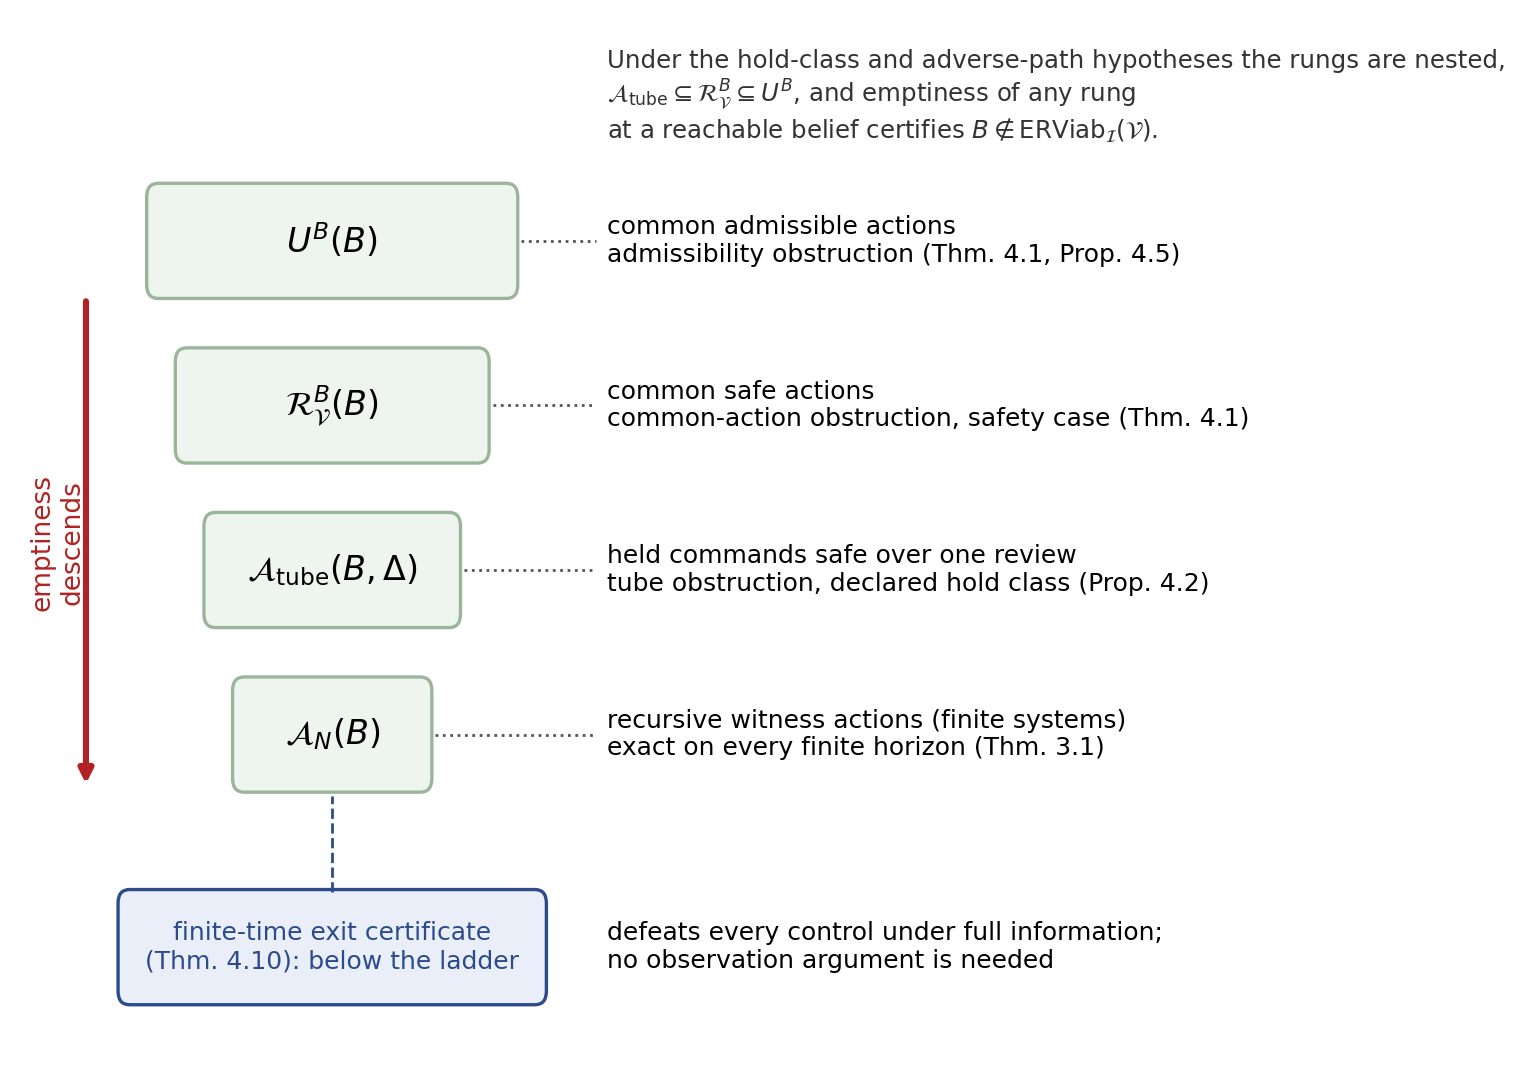
\includegraphics[width=0.9\textwidth]{figs/fig_v73_ladder.png}
\caption{The obstruction ladder (Proposition~4.2). The common response sets are nested, $U^B(B)\supseteq\cR^B_\cV(B)\supseteq\Atube(B,\Delta)$, under the hold-class and adverse-path hypotheses, and emptiness descends; the discrete $\cA_N$ joins the ladder only through a sampled-transition model; the finite-time exit certificate (Theorem~4.10) sits below the ladder because it defeats every control under full information.}
\label{fig:ladder}
\end{figure}

\begin{figure}[htbp]
\centering
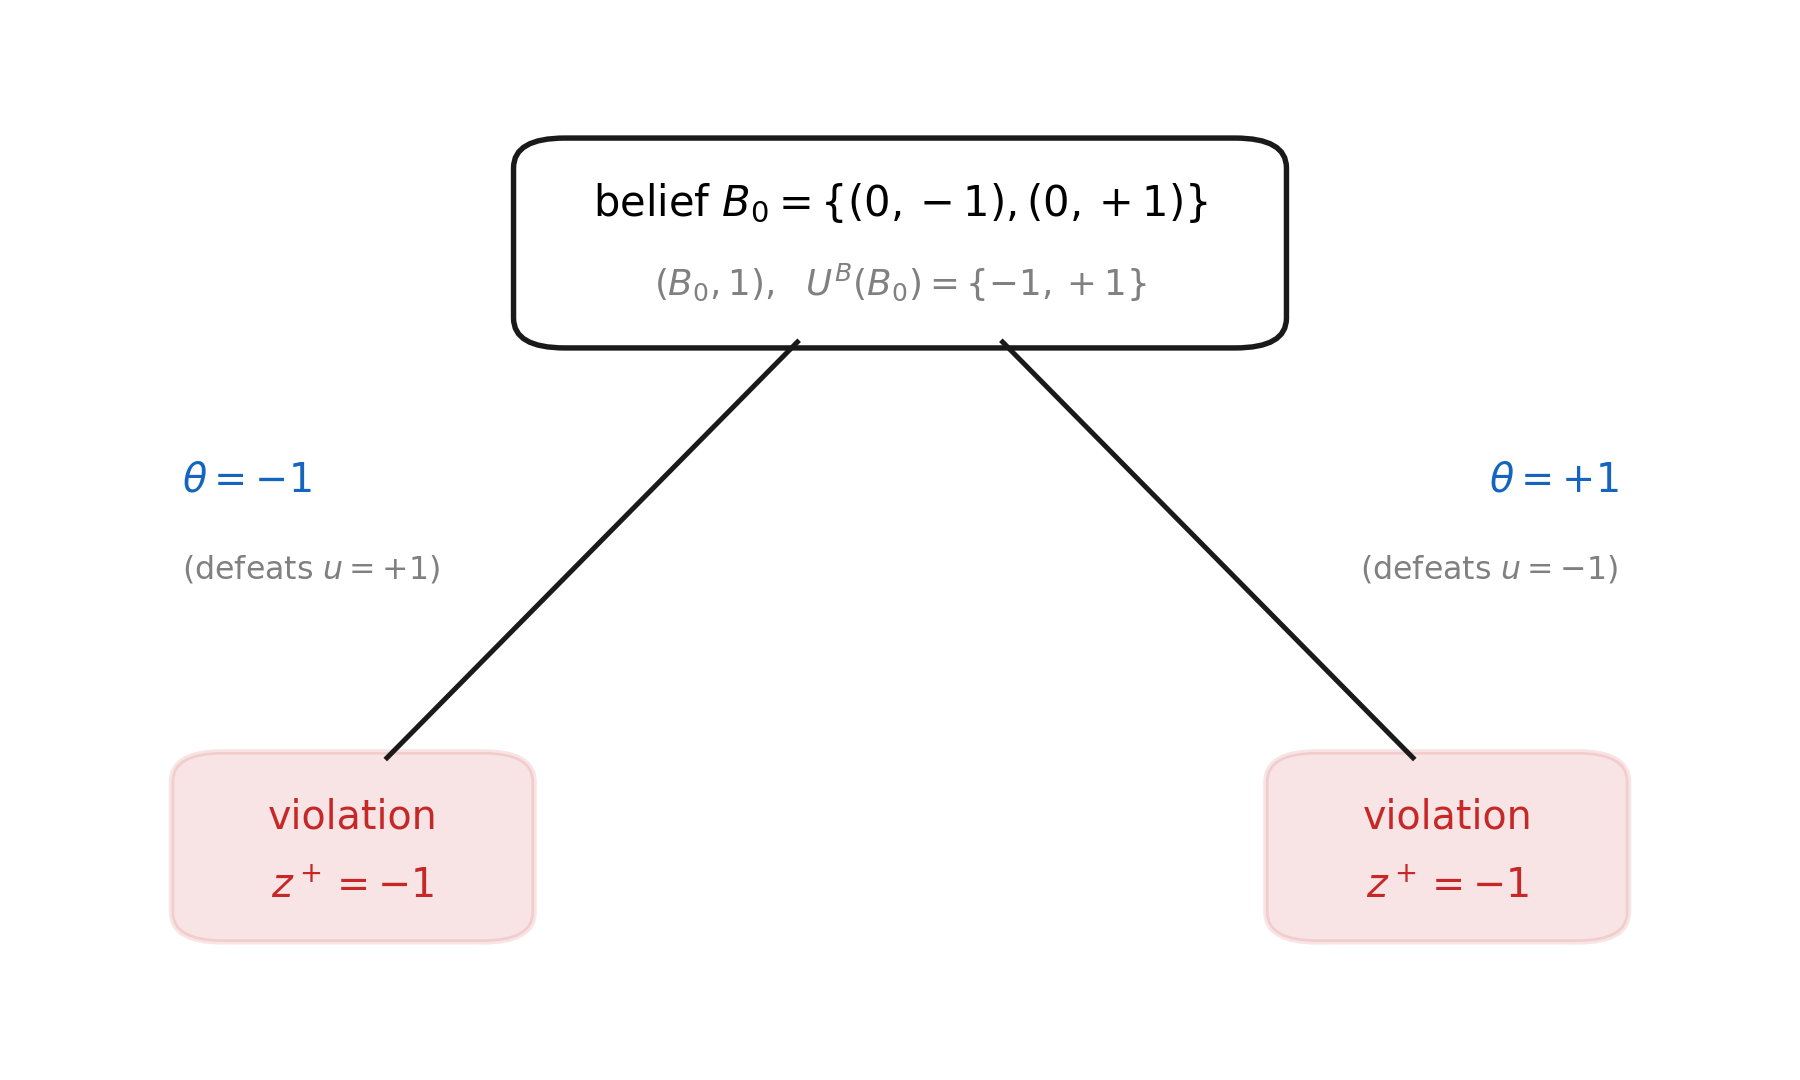
\includegraphics[width=0.62\textwidth]{figs/fig_p2_obstruction_tree.png}
\caption{The one-step obstruction tree of Example~3.3 read as a finite system (\S\ref{S:trees}): for each admissible action the adversary has a compatible branch terminating in violation, so $B_0\notin\cW_1$ (Theorem~3.1); the tree is the Lean term witnessing \texttt{hidden\_mode\_conflict}.}
\label{fig:tree}
\end{figure}

\begin{figure}[htbp]
\centering
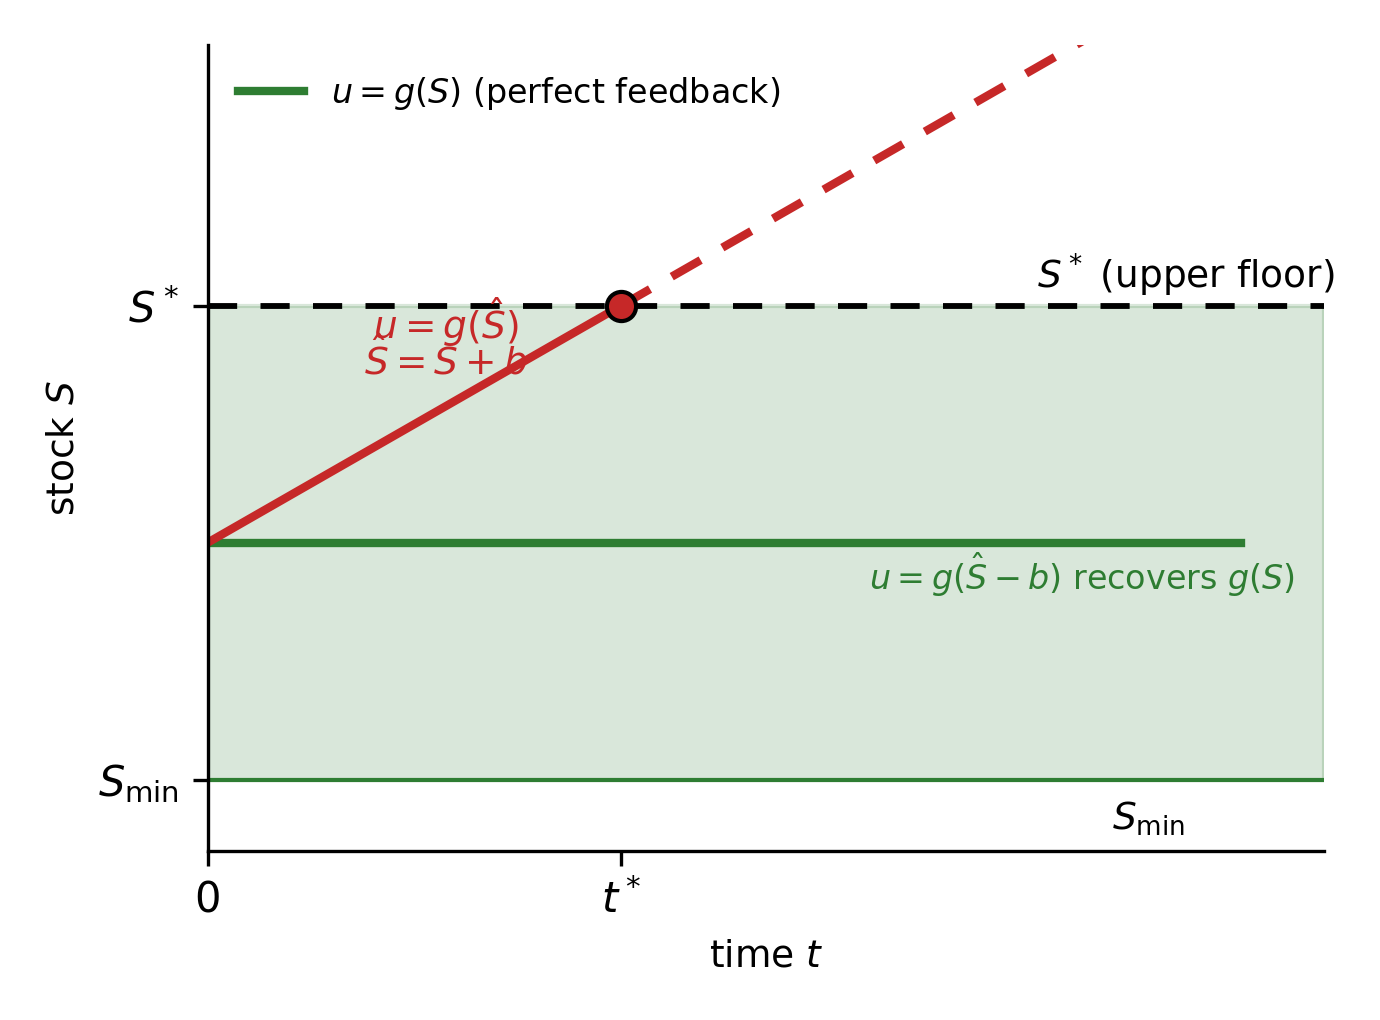
\includegraphics[width=0.6\textwidth]{figs/fig_p2_ce_trap.png}
\caption{The certainty-equivalence trap (Proposition~5.4). Under the perfect-information law $u=g(S)$ the stock is stationary inside $\cV$; the same law applied to the biased observation, $u=g(\hat S)$ with $\hat S=S+b$, gives $\dot S=g(S+b)-g(S)>0$ and exits above $S^*$ in finite time; inverting the bias restores $g(S)$.}
\label{fig:cetrap}
\end{figure}

\begin{figure}[htbp]
\centering
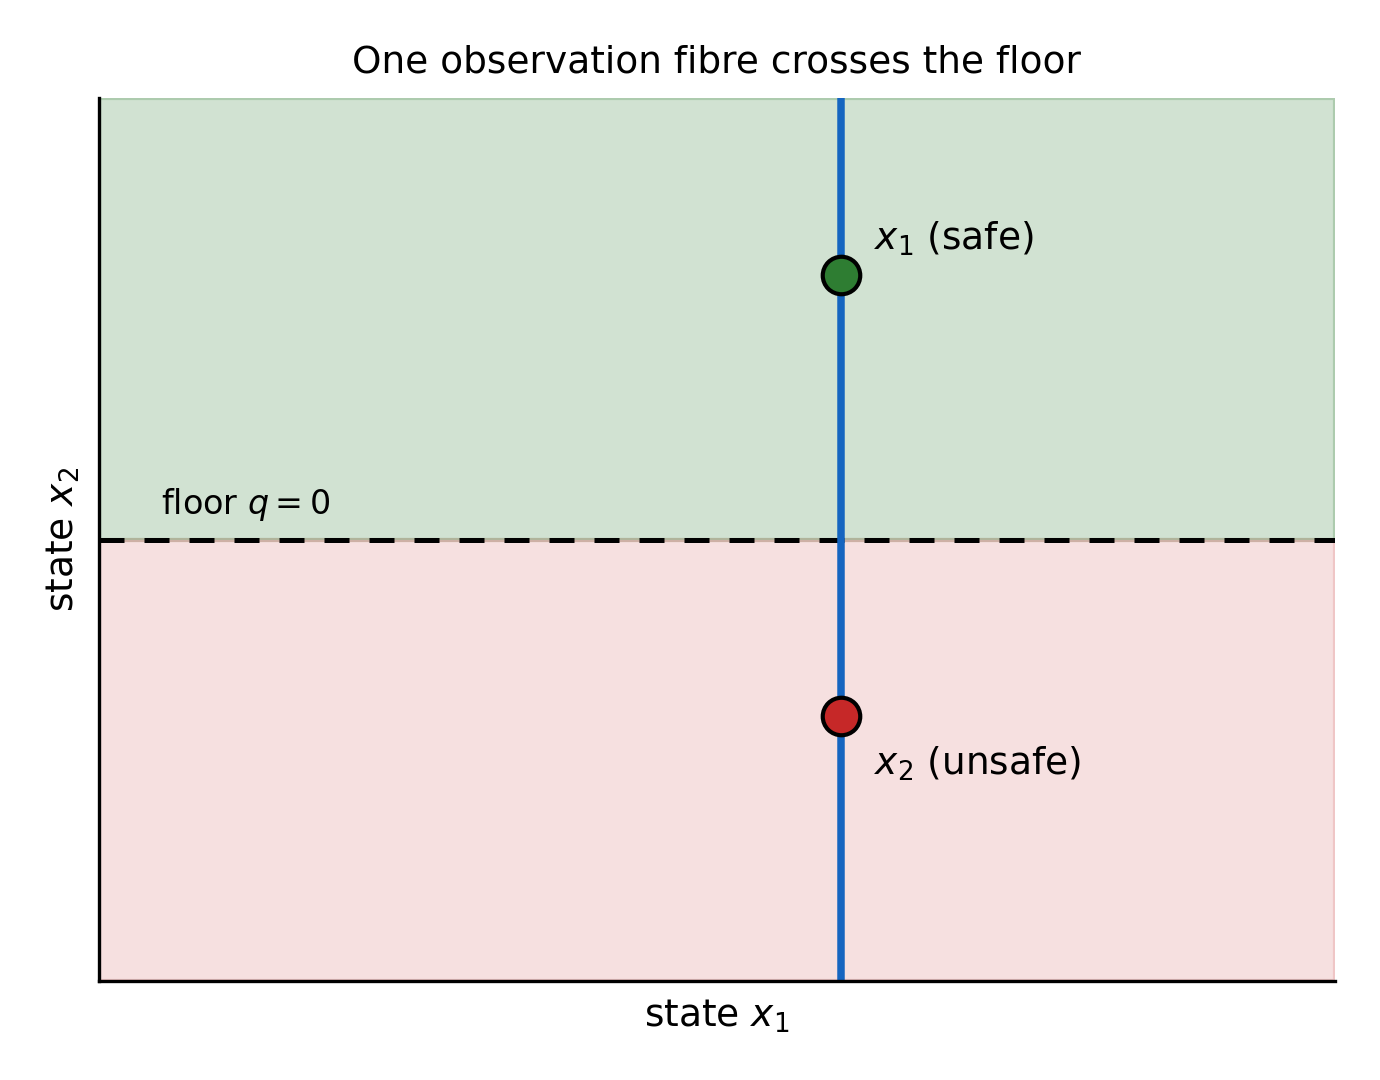
\includegraphics[width=0.72\textwidth]{figs/fig_p2_fibre.png}
\caption{An observation fibre crossing a floor boundary (Proposition~5.2, Corollary~5.3). The observation $O(x)=x_1$ cannot separate the safe state $(0.6,0.8)$ from the unsafe state $(0.6,0.3)$ on the same fibre, so no exact observation-only certifier exists; the certainly-safe readings are those whose entire fibre lies above the floor.}
\label{fig:fibre}
\end{figure}
\section{Result map}\label{S:map}

\begin{table}[htbp]
\centering\small
\begin{tabularx}{\textwidth}{@{}>{\raggedright\arraybackslash}p{0.17\textwidth}>{\raggedright\arraybackslash}X>{\raggedright\arraybackslash}p{0.13\textwidth}>{\raggedright\arraybackslash}p{0.30\textwidth}@{}}
\toprule
Result & Statement & Proof & Verification\\
\midrule
Prop.~2.2 & selector principle & \S\ref{S:selector} & ---\\
Thm.~3.1 & finite-horizon soundness and completeness & \S\ref{S:trees} & Lean \texttt{finite\_horizon\_*}\\
Thm.~3.2 & one-step completeness & main text & Lean \texttt{onestep\_char}\\
Ex.~3.3 & hidden-mode conflict & \S\ref{S:trees} & V10; Lean \texttt{hidden\_mode\_conflict}\\
Thm.~4.1 & common-action obstruction & \S\ref{S:common} & V1; Lean \texttt{common\_action\_obstruction}\\
Prop.~4.2 & obstruction ladder & \S\ref{S:common} & ---\\
Prop.~4.3 & sparse witness & \S\ref{S:helly} & ---\\
Rem.~4.4 & nonconvex counterexample; window rank & main text & ---\\
Prop.~4.5 & minimal admissibility construction & \S\ref{S:emptiness} & ---\\
Thm.~4.6 & delayed-information obstruction & \S\ref{S:delayed} & ---\\
Rem.~4.7 & threshold form & \S\ref{S:delayed} & ---\\
Thm.~4.8 & LP instantiation & \S\ref{S:lp} & V2, V3\\
Ex.~4.9 & decaying threshold; hold-class gap & \S\ref{S:lp} & V2, V3\\
Thm.~4.10 & finite-time exit & \S\ref{S:recourse} & ---\\
Rem.~4.11 & comparison form & \S\ref{S:recourse} & ---\\
Prop.~4.12 & oracle-recourse obstruction & \S\ref{S:recourse} & \texttt{counterexamples.py}\\
Ex.~4.13 & three-branch instance & \S\ref{S:threebranch} & V5\\
Prop.~5.2, Cor.~5.3 & fibre criterion; certainly-safe set & \S\ref{S:cert} & Lean \texttt{fibre\_criterion}, \texttt{crossing\_denies}\\
Prop.~5.4 & certainty-equivalence trap & \S\ref{S:cert} & V7\\
Thm.~6.1 & static-observation reduction & \S\ref{S:completeness} & ---\\
Prop.~6.2 & two-phase decomposition & \S\ref{S:completeness} & V9\\
Prop.~6.3 & window no-go & \S\ref{S:completeness}, \S\ref{S:A3} & V9\\
Prop.~6.4 & monotonicity & \S\ref{S:completeness} & Lean \texttt{Wk\_mono\_*}\\
Table~1, Fig.~5, Rem.~7.1 & coverage audit & \S\ref{S:holdclass} & V4\\
Table~2 & two-patch fibres & main text & V8\\
Section~7 (CE trap, aggregation) & worked instances & \S\ref{S:cert}, \S\ref{S:aggregateLP} & V6, V7\\
Thm.~\ref{thm:pomdp}, Props.~\ref{prop:chance}--\ref{prop:degenerate} & probabilistic counterpart & \S\ref{S:prob} & V4 (hold-class slice)\\
\S\ref{S:A1}--\S\ref{S:A2} & coupling constructions & \S\ref{S:constructions} & V11\\
\bottomrule
\end{tabularx}
\caption{Where each result is stated, proved and verified.}
\label{tab:map}
\end{table}

\renewcommand{\refname}{References}
\begin{thebibliography}{99}
\small
\bibitem[Abaee(2026)]{abaee2026aggregate} Abaee, A.: Aggregate indices and transition safety: a quantifier-order separation between scalarized and coordinate-wise feasibility. figshare, \url{https://doi.org/10.6084/m9.figshare.33764023} (2026)
\bibitem[\r{A}str\"om(1965)]{astrom1965} \r{A}str\"om, K.J.: Optimal control of Markov processes with incomplete state information. J. Math. Anal. Appl. \textbf{10}, 174--205 (1965)
\bibitem[Aubin(1991)]{aubin1991} Aubin, J.-P.: Viability Theory. Birkh\"auser, Boston (1991)
\bibitem[Cardaliaguet et~al.(2007)]{cardaliaguet2007} Cardaliaguet, P., Quincampoix, M., Saint-Pierre, P.: Differential games through viability theory: old and recent results. In: Advances in Dynamic Game Theory, Ann. Int. Soc. Dyn. Games, vol.~9, pp.~3--35. Birkh\"auser, Boston (2007)
\bibitem[Farkas(1902)]{farkas1902} Farkas, J.: Theorie der einfachen Ungleichungen. J. Reine Angew. Math. \textbf{124}, 1--27 (1902)
\bibitem[Gale(1960)]{gale1960} Gale, D.: The Theory of Linear Economic Models. McGraw-Hill, New York (1960)
\bibitem[Haddad(1981)]{haddad1981} Haddad, G.: Monotone viable trajectories for functional-differential inclusions. J. Differ. Equ. \textbf{42}, 1--24 (1981)
\bibitem[Helly(1923)]{helly1923} Helly, E.: \"Uber Mengen konvexer K\"orper mit gemeinschaftlichen Punkten. Jahresber. Dtsch. Math.-Ver. \textbf{32}, 175--176 (1923)
\bibitem[Kurzhanski and V\'alyi(1997)]{kurzhanski1997} Kurzhanski, A.B., V\'alyi, I.: Ellipsoidal Calculus for Estimation and Control. Birkh\"auser, Boston (1997)
\bibitem[Lovejoy(1991)]{lovejoy1991} Lovejoy, W.S.: Computationally feasible bounds for partially observed Markov decision processes. Oper. Res. \textbf{39}(1), 162--175 (1991)
\bibitem[Nagumo(1942)]{nagumo1942} Nagumo, M.: \"Uber die Lage der Integralkurven gew\"ohnlicher Differentialgleichungen. Proc. Phys.-Math. Soc. Japan \textbf{24}, 551--559 (1942)
\bibitem[Nakao et~al.(2021)]{nakao2021} Nakao, H., Jiang, R., Shen, S.: Distributionally robust partially observable Markov decision process with moment-based ambiguity. SIAM J. Optim. \textbf{31}(1), 461--488 (2021)
\bibitem[Papadimitriou and Tsitsiklis(1987)]{papadimitriou1987} Papadimitriou, C.H., Tsitsiklis, J.N.: The complexity of Markov decision processes. Math. Oper. Res. \textbf{12}(3), 441--450 (1987)
\bibitem[Smallwood and Sondik(1973)]{smallwood1973} Smallwood, R.D., Sondik, E.J.: The optimal control of partially observable Markov processes over a finite horizon. Oper. Res. \textbf{21}(5), 1071--1088 (1973)
\bibitem[Veliov(1993)]{veliov1993} Veliov, V.M.: Sufficient conditions for viability under imperfect measurement. Set-Valued Anal. \textbf{1}, 305--317 (1993)
\end{thebibliography}

\end{document}
